% Chapter 4: Probability
% Statistics of Financial Markets -- Bachelor's programme, Bucharest University of Economic Studies
% GENERATED by latex/build_chapter4.py -- edit the generator, not this file.

\newcommand{\coursename}{Statistics of Financial Markets}
% Preambul comun SFM -- Statistica piețelor financiare / Statistics of Financial Markets (Beamer, 16:9)
% Același design ca MFM. Înainte de % Preambul comun SFM -- Statistica piețelor financiare / Statistics of Financial Markets (Beamer, 16:9)
% Același design ca MFM. Înainte de % Preambul comun SFM -- Statistica piețelor financiare / Statistics of Financial Markets (Beamer, 16:9)
% Același design ca MFM. Înainte de \input{../../latex/preamble} se definește
%   \newcommand{\coursename}{Statistics of Financial Markets}      (EN)
%   \newcommand{\coursename}{Statistica piețelor financiare}       (RO)  și  \def\sfmlang{ro}
% Fișierele .tex se află în EN/Courses, EN/Seminars, RO/Cursuri, RO/Seminarii (două niveluri sub rădăcină).
% Deck-urile sînt generate de latex/build_chapterN.py / build_seminarN.py (vezi latex/sfm_build.py).

\documentclass[9pt, aspectratio=169, t]{beamer}
\providecommand{\coursename}{Statistics of Financial Markets}

% Ensure content fits on slides
\setbeamersize{text margin left=8mm, text margin right=8mm}

%=============================================================================
% THEME AND STYLE CONFIGURATION
%=============================================================================
\usetheme{default}
% Using default theme for clean header/footer control

% Color Palette (matching Redispatch PDF)
\definecolor{MainBlue}{RGB}{26, 58, 110}
\definecolor{AccentBlue}{RGB}{26, 58, 110}
\definecolor{IDAred}{RGB}{205, 0, 0}
\definecolor{DarkGray}{RGB}{51, 51, 51}
\definecolor{MediumGray}{RGB}{128, 128, 128}
\definecolor{LightGray}{RGB}{248, 248, 248}
\definecolor{VeryLightGray}{RGB}{235, 235, 235}
\definecolor{KeynoteGray}{RGB}{218, 218, 218}
\definecolor{SectionGray}{RGB}{120, 120, 120}
\definecolor{FooterGray}{RGB}{100, 100, 100}
\definecolor{Crimson}{RGB}{220, 53, 69}
\definecolor{Forest}{RGB}{46, 125, 50}
\definecolor{Amber}{RGB}{181, 133, 63}
\definecolor{Orange}{RGB}{230, 126, 34}
\definecolor{Purple}{RGB}{142, 68, 173}

% Gradient background (exact Keynote 315° gradient: white to RGB 218,218,218)
\setbeamertemplate{background}{%
    \begin{tikzpicture}[remember picture, overlay]
        \shade[shading=axis, shading angle=315,
        top color=white, bottom color=KeynoteGray]
        (current page.south west) rectangle (current page.north east);
    \end{tikzpicture}%
}
% Fallback solid color for compatibility
\setbeamercolor{background canvas}{bg=}

\setbeamercolor{palette primary}{bg=MainBlue, fg=white}
\setbeamercolor{palette secondary}{bg=MainBlue!85, fg=white}
\setbeamercolor{palette tertiary}{bg=MainBlue!70, fg=white}
\setbeamercolor{structure}{fg=MainBlue}
\setbeamercolor{title}{fg=IDAred}
\setbeamercolor{frametitle}{fg=IDAred, bg=}
\setbeamercolor{block title}{bg=MainBlue, fg=white}
\setbeamercolor{block body}{bg=VeryLightGray, fg=DarkGray}
\setbeamercolor{block title alerted}{bg=Crimson, fg=white}
\setbeamercolor{block body alerted}{bg=Crimson!8, fg=DarkGray}
\setbeamercolor{block title example}{bg=Forest, fg=white}
\setbeamercolor{block body example}{bg=Forest!8, fg=DarkGray}
\setbeamercolor{item}{fg=MainBlue}

% Footer colors (override Madrid theme blue)
\setbeamercolor{author in head/foot}{fg=FooterGray, bg=}
\setbeamercolor{title in head/foot}{fg=FooterGray, bg=}
\setbeamercolor{date in head/foot}{fg=FooterGray, bg=}
\setbeamercolor{section in head/foot}{fg=FooterGray, bg=}
\setbeamercolor{subsection in head/foot}{fg=FooterGray, bg=}

% Bullet styles (apply everywhere including blocks)
\setbeamertemplate{itemize item}{\color{MainBlue}$\boxdot$}
\setbeamertemplate{itemize subitem}{\color{MainBlue}$\blacktriangleright$}
\setbeamertemplate{itemize subsubitem}{\color{MainBlue}\tiny$\bullet$}
\setbeamertemplate{itemize/enumerate body begin}{\normalsize}
\setbeamertemplate{itemize/enumerate subbody begin}{\normalsize}

% Item spacing - compact style
\setlength{\leftmargini}{10pt}       % Level 1: minimal indent
\setlength{\leftmarginii}{10pt}      % Level 2: minimal additional indent
% Compact list spacing (zero extra space before/after lists in blocks)
\makeatletter
\def\@listi{\leftmargin\leftmargini \topsep 0pt \parsep 0pt \itemsep 0pt}
\def\@listii{\leftmargin\leftmarginii \topsep 0pt \parsep 0pt \itemsep 0pt}
\makeatother

\setbeamertemplate{navigation symbols}{}

%=============================================================================
% CUSTOM HEADLINE
%=============================================================================
\setbeamertemplate{headline}{%
    \vskip10pt%
    \hbox to \paperwidth{%
        \hskip0.5cm%
        {\small\color{FooterGray}\renewcommand{\hyperlink}[2]{##2}\insertsectionhead}%
        \hfill%
        \textcolor{FooterGray}{\small\insertframenumber}%
        \hskip0.5cm%
    }%
    \vskip4pt%
    {\color{FooterGray}\hrule height 0.4pt}%
}

%=============================================================================
% CUSTOM FOOTER
%=============================================================================
\usepackage{fontawesome5}

\setbeamertemplate{footline}{%
    {\color{FooterGray}\hrule height 0.4pt}%
    \vskip4pt%
    \hbox to \paperwidth{%
        \hskip0.5cm%
        \textcolor{FooterGray}{\small\coursename}%
        \hfill%
        \raisebox{-0.1em}{%
            \begin{tikzpicture}[x=0.08em, y=0.08em, line width=0.4pt]
                \draw[FooterGray] (0,3) -- (1,4) -- (2,3.5) -- (3,5) -- (4,4) -- (5,6) -- (6,5.5) -- (7,4) -- (8,5) -- (9,7) -- (10,6) -- (11,5) -- (12,6.5) -- (13,8) -- (14,7) -- (15,6) -- (16,7.5) -- (17,9) -- (18,8) -- (19,7) -- (20,8.5) -- (21,10) -- (22,9) -- (23,8) -- (24,9.5);
            \end{tikzpicture}%
        }%
        \hskip0.5cm%
    }%
    \vskip6pt%
}

%=============================================================================
% PACKAGES
%=============================================================================
\usepackage[utf8]{inputenc}
\DeclareUnicodeCharacter{03B1}{\ensuremath{\alpha}}
\usepackage[T1]{fontenc}
\usepackage{amsmath, amssymb, amsthm}
\usepackage{mathtools}
\usepackage{bm}
\usepackage{tikz}
\usetikzlibrary{arrows.meta, positioning, shapes, calc, decorations.pathreplacing, shadings}
\usepackage{booktabs}
\usepackage{multirow}
\usepackage{array}
\usepackage{graphicx}
\usepackage{hyperref}
\usepackage{colortbl}
\usepackage{listings}
\lstset{language=Python, basicstyle=\ttfamily\scriptsize, keywordstyle=\color{MainBlue}\bfseries,
  commentstyle=\color{Forest}, stringstyle=\color{Crimson}, breaklines=true,
  frame=none, backgroundcolor=\color{VeryLightGray}, xleftmargin=2mm}
\hypersetup{colorlinks=true, linkcolor=MainBlue, urlcolor=MainBlue}
\graphicspath{{../../logos/}{../../charts/}{../../photos/}}
\usepackage{xcolor}
\hfuzz=2pt  % Suppress tiny overfull warnings (<2pt)
\vfuzz=2pt  % Suppress tiny vertical overfull warnings (<2pt)

%=============================================================================
% QUANTLET COMMANDS
%   \quantlet{<displayed name>}{<url>}       (generic, compatible with the older SFM decks)
%   \sfmquantlet{Ch_05}{SFM_ch5_garch}       -> https://github.com/danpele/SFM/tree/main/Quantlets/Ch_05/SFM_ch5_garch
%   \qlurl{<folder>} is defined per chapter by the generator (Quantlets/Ch_NN/<folder>)
%=============================================================================
\newcommand{\sfmrepo}{https://github.com/danpele/SFM}
\newcommand{\sfmqlbase}{https://github.com/danpele/SFM/tree/main/Quantlets}
\newcommand{\quantlet}[2]{%
    \hfill\href{#2}{%
        \raisebox{-0.15em}{
\includegraphics[height=0.7em]{ql_logo.png}}%
        \textcolor{MainBlue}{\tiny\ #1}%
    }%
}
\newcommand{\sfmquantlet}[2]{\quantlet{\detokenize{#2}}{\sfmqlbase/#1/#2}}

%=============================================================================
% NOTEBOOKS (Google Colab)
%   \colaburl{notebooks/EN/chapter5_seminar_notebook.ipynb} -> the Colab link of a file in the SFM repo
%   \nb: the chapter notebook (each seminar deck redefines it with \renewcommand)
%=============================================================================
\newcommand{\colaburl}[1]{https://colab.research.google.com/github/danpele/SFM/blob/main/#1}
\newcommand{\nb}{https://colab.research.google.com/github/danpele/SFM/tree/main/notebooks/EN}
\newcommand{\nbname}{notebooks/EN}

%=============================================================================
% SLIDE HELPERS (used by the generators; the same as in MFM)
%=============================================================================
% local font size for list bodies (the preamble forces \normalsize)
\newcommand{\itemsize}[1]{\setbeamertemplate{itemize/enumerate body begin}{#1}\setbeamertemplate{itemize/enumerate subbody begin}{#1}}
\newcommand{\intitle}[1]{{\hypersetup{urlcolor=white}#1}}   % white links inside coloured title bars
\newcommand{\imgcap}[1]{{\scriptsize #1}\\[0.5mm]}          % caption under a photo
\newcommand{\imgcredit}[2]{{\tiny\color{FooterGray}\href{#1}{#2}}}   % image credit: source URL, author/licence
\newcommand{\aiprompt}[1]{{\ttfamily\color{MainBlue}#1}}     % a prompt to an AI assistant

%=============================================================================
% SEMINARS: student version by default; the instructor wrapper *_solutions.tex sets \solutionstrue
%=============================================================================
\makeatletter\@ifundefined{ifsolutions}{\expandafter\newif\csname ifsolutions\endcsname}{}\makeatother
\newcommand{\solonly}[1]{\ifsolutions #1\fi}
\newcommand{\propsub}{\ifsolutions\else\framesubtitle{\ifdefined\sfmlang Rezolvarea se discută la seminar\else Solution discussed in class\fi}\fi}

%=============================================================================
% APPENDIX AND CHAPTER LINKS (latex/appendix_links.py writes the calls; it also re-declares these
% macros before \begin{document}, so the decks compile with or without this preamble block)
%=============================================================================
\providecommand{\sfmapplink}[3]{\hypertarget{#2}{}\hyperlink{#1}{\beamergotobutton{#3}}}
\providecommand{\sfmappback}[2]{\begin{tikzpicture}[remember picture,overlay]\node[anchor=south east] at ([xshift=-3mm,yshift=7mm]current page.south east){\hyperlink{#1}{\beamerreturnbutton{#2}}};\end{tikzpicture}}
\providecommand{\sfmchlink}[2]{\href{#1}{#2}}
\providecommand{\sfmchlinkt}[2]{\href{#1}{\usebeamercolor[fg]{frametitle}#2}}

%=============================================================================
% QUANTINAR COMMAND: link către un curs Quantinar (subiecte avansate)
%=============================================================================
\newcommand{\quantinar}[2]{%
    \href{#2}{%
        \raisebox{-0.15em}{
\includegraphics[height=0.8em]{qr_logo.png}}%
        \textcolor{MainBlue}{\scriptsize\ #1}%
    }%
}

%=============================================================================
% CUSTOM TITLE PAGE
%=============================================================================
\defbeamertemplate*{title page}{hybrid}[1][]
{
    \vspace{0.2cm}
    % Logos row - top header (with clickable links)
    \begin{center}
        \href{https://www.ase.ro}{
\includegraphics[height=1.0cm]{ase_logo.png}}\hspace{0.3cm}%
        \href{https://theida.net}{
\includegraphics[height=1.0cm]{ida_logo.png}}\hspace{0.3cm}%
        \href{https://blockchain-research-center.com}{
\includegraphics[height=1.0cm]{brc_logo.png}}\hspace{0.3cm}%
        \href{https://www.ai4efin.ase.ro}{
\includegraphics[height=1.0cm]{ai4efin_logo.png}}\hspace{0.3cm}%
        \href{https://ipe.ro/new}{
\includegraphics[height=1.0cm]{acad_logo.png}}\hspace{0.3cm}%
        \href{https://www.digital-finance-msca.com}{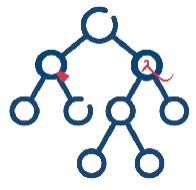
\includegraphics[height=1.0cm]{msca_logo.png}}%
    \end{center}

    \vspace{0.6cm}

    % Main title with Q logos on sides (with clickable links)
    \begin{center}
        \begin{minipage}{0.1\textwidth}
            \centering
            \href{https://quantlet.com}{
\includegraphics[height=1.1cm]{ql_logo.png}}
        \end{minipage}%
        \begin{minipage}{0.78\textwidth}
            \centering
            {\LARGE\bfseries\usebeamercolor[fg]{title}\inserttitle}

            \vspace{0.3cm}

            {\usebeamerfont{subtitle}\usebeamercolor[fg]{title}\insertsubtitle}
        \end{minipage}%
        \begin{minipage}{0.1\textwidth}
            \centering
            \href{https://quantinar.com}{
\includegraphics[height=1.1cm]{qr_logo.png}}
        \end{minipage}
    \end{center}

    \vspace{0.6cm}

    % Authors (left aligned)
    \hspace{0.5cm}{\usebeamerfont{author}\insertauthor}

    \vspace{0.3cm}

    % Institute/Affiliations (left aligned)
    \hspace{0.5cm}\begin{minipage}[t]{0.9\textwidth}
        \raggedright\small\insertinstitute
    \end{minipage}
}

%=============================================================================
% THEOREM ENVIRONMENTS
%=============================================================================
\theoremstyle{definition}
\setbeamertemplate{theorems}[numbered]
\ifdefined\sfmlang
\newtheorem{defn}{Definiție}
\newtheorem{thm}{Teoremă}
\newtheorem{prop}{Propoziție}
\newtheorem{rmk}{Observație}
\else
\newtheorem{defn}{Definition}
\newtheorem{thm}{Theorem}
\newtheorem{prop}{Proposition}
\newtheorem{rmk}{Remark}
\fi

%=============================================================================
% CENTRED MINIPAGE (no extra vertical space)
%=============================================================================
\newenvironment{cminipage}[1]{%
    \par\noindent\hfill\begin{minipage}{#1}\ignorespaces
}{%
    \end{minipage}\hfill\null\par
}

%=============================================================================
% CUSTOM COMMANDS
%=============================================================================
\newcommand{\E}{\mathbb{E}}
\newcommand{\Var}{\text{Var}}
\newcommand{\Cov}{\text{Cov}}
\newcommand{\Corr}{\text{Corr}}
\newcommand{\R}{\mathbb{R}}
\newcommand{\N}{\mathbb{N}}
\newcommand{\Z}{\mathbb{Z}}
\newcommand{\B}{\mathbf{B}}
\newcommand{\imark}{\textcolor{MainBlue}{\textbullet}}
\newcommand{\RMSE}{\text{RMSE}}
\newcommand{\MAE}{\text{MAE}}
\newcommand{\MAPE}{\text{MAPE}}

 se definește
%   \newcommand{\coursename}{Statistics of Financial Markets}      (EN)
%   \newcommand{\coursename}{Statistica piețelor financiare}       (RO)  și  \def\sfmlang{ro}
% Fișierele .tex se află în EN/Courses, EN/Seminars, RO/Cursuri, RO/Seminarii (două niveluri sub rădăcină).
% Deck-urile sînt generate de latex/build_chapterN.py / build_seminarN.py (vezi latex/sfm_build.py).

\documentclass[9pt, aspectratio=169, t]{beamer}
\providecommand{\coursename}{Statistics of Financial Markets}

% Ensure content fits on slides
\setbeamersize{text margin left=8mm, text margin right=8mm}

%=============================================================================
% THEME AND STYLE CONFIGURATION
%=============================================================================
\usetheme{default}
% Using default theme for clean header/footer control

% Color Palette (matching Redispatch PDF)
\definecolor{MainBlue}{RGB}{26, 58, 110}
\definecolor{AccentBlue}{RGB}{26, 58, 110}
\definecolor{IDAred}{RGB}{205, 0, 0}
\definecolor{DarkGray}{RGB}{51, 51, 51}
\definecolor{MediumGray}{RGB}{128, 128, 128}
\definecolor{LightGray}{RGB}{248, 248, 248}
\definecolor{VeryLightGray}{RGB}{235, 235, 235}
\definecolor{KeynoteGray}{RGB}{218, 218, 218}
\definecolor{SectionGray}{RGB}{120, 120, 120}
\definecolor{FooterGray}{RGB}{100, 100, 100}
\definecolor{Crimson}{RGB}{220, 53, 69}
\definecolor{Forest}{RGB}{46, 125, 50}
\definecolor{Amber}{RGB}{181, 133, 63}
\definecolor{Orange}{RGB}{230, 126, 34}
\definecolor{Purple}{RGB}{142, 68, 173}

% Gradient background (exact Keynote 315° gradient: white to RGB 218,218,218)
\setbeamertemplate{background}{%
    \begin{tikzpicture}[remember picture, overlay]
        \shade[shading=axis, shading angle=315,
        top color=white, bottom color=KeynoteGray]
        (current page.south west) rectangle (current page.north east);
    \end{tikzpicture}%
}
% Fallback solid color for compatibility
\setbeamercolor{background canvas}{bg=}

\setbeamercolor{palette primary}{bg=MainBlue, fg=white}
\setbeamercolor{palette secondary}{bg=MainBlue!85, fg=white}
\setbeamercolor{palette tertiary}{bg=MainBlue!70, fg=white}
\setbeamercolor{structure}{fg=MainBlue}
\setbeamercolor{title}{fg=IDAred}
\setbeamercolor{frametitle}{fg=IDAred, bg=}
\setbeamercolor{block title}{bg=MainBlue, fg=white}
\setbeamercolor{block body}{bg=VeryLightGray, fg=DarkGray}
\setbeamercolor{block title alerted}{bg=Crimson, fg=white}
\setbeamercolor{block body alerted}{bg=Crimson!8, fg=DarkGray}
\setbeamercolor{block title example}{bg=Forest, fg=white}
\setbeamercolor{block body example}{bg=Forest!8, fg=DarkGray}
\setbeamercolor{item}{fg=MainBlue}

% Footer colors (override Madrid theme blue)
\setbeamercolor{author in head/foot}{fg=FooterGray, bg=}
\setbeamercolor{title in head/foot}{fg=FooterGray, bg=}
\setbeamercolor{date in head/foot}{fg=FooterGray, bg=}
\setbeamercolor{section in head/foot}{fg=FooterGray, bg=}
\setbeamercolor{subsection in head/foot}{fg=FooterGray, bg=}

% Bullet styles (apply everywhere including blocks)
\setbeamertemplate{itemize item}{\color{MainBlue}$\boxdot$}
\setbeamertemplate{itemize subitem}{\color{MainBlue}$\blacktriangleright$}
\setbeamertemplate{itemize subsubitem}{\color{MainBlue}\tiny$\bullet$}
\setbeamertemplate{itemize/enumerate body begin}{\normalsize}
\setbeamertemplate{itemize/enumerate subbody begin}{\normalsize}

% Item spacing - compact style
\setlength{\leftmargini}{10pt}       % Level 1: minimal indent
\setlength{\leftmarginii}{10pt}      % Level 2: minimal additional indent
% Compact list spacing (zero extra space before/after lists in blocks)
\makeatletter
\def\@listi{\leftmargin\leftmargini \topsep 0pt \parsep 0pt \itemsep 0pt}
\def\@listii{\leftmargin\leftmarginii \topsep 0pt \parsep 0pt \itemsep 0pt}
\makeatother

\setbeamertemplate{navigation symbols}{}

%=============================================================================
% CUSTOM HEADLINE
%=============================================================================
\setbeamertemplate{headline}{%
    \vskip10pt%
    \hbox to \paperwidth{%
        \hskip0.5cm%
        {\small\color{FooterGray}\renewcommand{\hyperlink}[2]{##2}\insertsectionhead}%
        \hfill%
        \textcolor{FooterGray}{\small\insertframenumber}%
        \hskip0.5cm%
    }%
    \vskip4pt%
    {\color{FooterGray}\hrule height 0.4pt}%
}

%=============================================================================
% CUSTOM FOOTER
%=============================================================================
\usepackage{fontawesome5}

\setbeamertemplate{footline}{%
    {\color{FooterGray}\hrule height 0.4pt}%
    \vskip4pt%
    \hbox to \paperwidth{%
        \hskip0.5cm%
        \textcolor{FooterGray}{\small\coursename}%
        \hfill%
        \raisebox{-0.1em}{%
            \begin{tikzpicture}[x=0.08em, y=0.08em, line width=0.4pt]
                \draw[FooterGray] (0,3) -- (1,4) -- (2,3.5) -- (3,5) -- (4,4) -- (5,6) -- (6,5.5) -- (7,4) -- (8,5) -- (9,7) -- (10,6) -- (11,5) -- (12,6.5) -- (13,8) -- (14,7) -- (15,6) -- (16,7.5) -- (17,9) -- (18,8) -- (19,7) -- (20,8.5) -- (21,10) -- (22,9) -- (23,8) -- (24,9.5);
            \end{tikzpicture}%
        }%
        \hskip0.5cm%
    }%
    \vskip6pt%
}

%=============================================================================
% PACKAGES
%=============================================================================
\usepackage[utf8]{inputenc}
\DeclareUnicodeCharacter{03B1}{\ensuremath{\alpha}}
\usepackage[T1]{fontenc}
\usepackage{amsmath, amssymb, amsthm}
\usepackage{mathtools}
\usepackage{bm}
\usepackage{tikz}
\usetikzlibrary{arrows.meta, positioning, shapes, calc, decorations.pathreplacing, shadings}
\usepackage{booktabs}
\usepackage{multirow}
\usepackage{array}
\usepackage{graphicx}
\usepackage{hyperref}
\usepackage{colortbl}
\usepackage{listings}
\lstset{language=Python, basicstyle=\ttfamily\scriptsize, keywordstyle=\color{MainBlue}\bfseries,
  commentstyle=\color{Forest}, stringstyle=\color{Crimson}, breaklines=true,
  frame=none, backgroundcolor=\color{VeryLightGray}, xleftmargin=2mm}
\hypersetup{colorlinks=true, linkcolor=MainBlue, urlcolor=MainBlue}
\graphicspath{{../../logos/}{../../charts/}{../../photos/}}
\usepackage{xcolor}
\hfuzz=2pt  % Suppress tiny overfull warnings (<2pt)
\vfuzz=2pt  % Suppress tiny vertical overfull warnings (<2pt)

%=============================================================================
% QUANTLET COMMANDS
%   \quantlet{<displayed name>}{<url>}       (generic, compatible with the older SFM decks)
%   \sfmquantlet{Ch_05}{SFM_ch5_garch}       -> https://github.com/danpele/SFM/tree/main/Quantlets/Ch_05/SFM_ch5_garch
%   \qlurl{<folder>} is defined per chapter by the generator (Quantlets/Ch_NN/<folder>)
%=============================================================================
\newcommand{\sfmrepo}{https://github.com/danpele/SFM}
\newcommand{\sfmqlbase}{https://github.com/danpele/SFM/tree/main/Quantlets}
\newcommand{\quantlet}[2]{%
    \hfill\href{#2}{%
        \raisebox{-0.15em}{
\includegraphics[height=0.7em]{ql_logo.png}}%
        \textcolor{MainBlue}{\tiny\ #1}%
    }%
}
\newcommand{\sfmquantlet}[2]{\quantlet{\detokenize{#2}}{\sfmqlbase/#1/#2}}

%=============================================================================
% NOTEBOOKS (Google Colab)
%   \colaburl{notebooks/EN/chapter5_seminar_notebook.ipynb} -> the Colab link of a file in the SFM repo
%   \nb: the chapter notebook (each seminar deck redefines it with \renewcommand)
%=============================================================================
\newcommand{\colaburl}[1]{https://colab.research.google.com/github/danpele/SFM/blob/main/#1}
\newcommand{\nb}{https://colab.research.google.com/github/danpele/SFM/tree/main/notebooks/EN}
\newcommand{\nbname}{notebooks/EN}

%=============================================================================
% SLIDE HELPERS (used by the generators; the same as in MFM)
%=============================================================================
% local font size for list bodies (the preamble forces \normalsize)
\newcommand{\itemsize}[1]{\setbeamertemplate{itemize/enumerate body begin}{#1}\setbeamertemplate{itemize/enumerate subbody begin}{#1}}
\newcommand{\intitle}[1]{{\hypersetup{urlcolor=white}#1}}   % white links inside coloured title bars
\newcommand{\imgcap}[1]{{\scriptsize #1}\\[0.5mm]}          % caption under a photo
\newcommand{\imgcredit}[2]{{\tiny\color{FooterGray}\href{#1}{#2}}}   % image credit: source URL, author/licence
\newcommand{\aiprompt}[1]{{\ttfamily\color{MainBlue}#1}}     % a prompt to an AI assistant

%=============================================================================
% SEMINARS: student version by default; the instructor wrapper *_solutions.tex sets \solutionstrue
%=============================================================================
\makeatletter\@ifundefined{ifsolutions}{\expandafter\newif\csname ifsolutions\endcsname}{}\makeatother
\newcommand{\solonly}[1]{\ifsolutions #1\fi}
\newcommand{\propsub}{\ifsolutions\else\framesubtitle{\ifdefined\sfmlang Rezolvarea se discută la seminar\else Solution discussed in class\fi}\fi}

%=============================================================================
% APPENDIX AND CHAPTER LINKS (latex/appendix_links.py writes the calls; it also re-declares these
% macros before \begin{document}, so the decks compile with or without this preamble block)
%=============================================================================
\providecommand{\sfmapplink}[3]{\hypertarget{#2}{}\hyperlink{#1}{\beamergotobutton{#3}}}
\providecommand{\sfmappback}[2]{\begin{tikzpicture}[remember picture,overlay]\node[anchor=south east] at ([xshift=-3mm,yshift=7mm]current page.south east){\hyperlink{#1}{\beamerreturnbutton{#2}}};\end{tikzpicture}}
\providecommand{\sfmchlink}[2]{\href{#1}{#2}}
\providecommand{\sfmchlinkt}[2]{\href{#1}{\usebeamercolor[fg]{frametitle}#2}}

%=============================================================================
% QUANTINAR COMMAND: link către un curs Quantinar (subiecte avansate)
%=============================================================================
\newcommand{\quantinar}[2]{%
    \href{#2}{%
        \raisebox{-0.15em}{
\includegraphics[height=0.8em]{qr_logo.png}}%
        \textcolor{MainBlue}{\scriptsize\ #1}%
    }%
}

%=============================================================================
% CUSTOM TITLE PAGE
%=============================================================================
\defbeamertemplate*{title page}{hybrid}[1][]
{
    \vspace{0.2cm}
    % Logos row - top header (with clickable links)
    \begin{center}
        \href{https://www.ase.ro}{
\includegraphics[height=1.0cm]{ase_logo.png}}\hspace{0.3cm}%
        \href{https://theida.net}{
\includegraphics[height=1.0cm]{ida_logo.png}}\hspace{0.3cm}%
        \href{https://blockchain-research-center.com}{
\includegraphics[height=1.0cm]{brc_logo.png}}\hspace{0.3cm}%
        \href{https://www.ai4efin.ase.ro}{
\includegraphics[height=1.0cm]{ai4efin_logo.png}}\hspace{0.3cm}%
        \href{https://ipe.ro/new}{
\includegraphics[height=1.0cm]{acad_logo.png}}\hspace{0.3cm}%
        \href{https://www.digital-finance-msca.com}{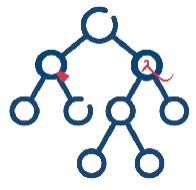
\includegraphics[height=1.0cm]{msca_logo.png}}%
    \end{center}

    \vspace{0.6cm}

    % Main title with Q logos on sides (with clickable links)
    \begin{center}
        \begin{minipage}{0.1\textwidth}
            \centering
            \href{https://quantlet.com}{
\includegraphics[height=1.1cm]{ql_logo.png}}
        \end{minipage}%
        \begin{minipage}{0.78\textwidth}
            \centering
            {\LARGE\bfseries\usebeamercolor[fg]{title}\inserttitle}

            \vspace{0.3cm}

            {\usebeamerfont{subtitle}\usebeamercolor[fg]{title}\insertsubtitle}
        \end{minipage}%
        \begin{minipage}{0.1\textwidth}
            \centering
            \href{https://quantinar.com}{
\includegraphics[height=1.1cm]{qr_logo.png}}
        \end{minipage}
    \end{center}

    \vspace{0.6cm}

    % Authors (left aligned)
    \hspace{0.5cm}{\usebeamerfont{author}\insertauthor}

    \vspace{0.3cm}

    % Institute/Affiliations (left aligned)
    \hspace{0.5cm}\begin{minipage}[t]{0.9\textwidth}
        \raggedright\small\insertinstitute
    \end{minipage}
}

%=============================================================================
% THEOREM ENVIRONMENTS
%=============================================================================
\theoremstyle{definition}
\setbeamertemplate{theorems}[numbered]
\ifdefined\sfmlang
\newtheorem{defn}{Definiție}
\newtheorem{thm}{Teoremă}
\newtheorem{prop}{Propoziție}
\newtheorem{rmk}{Observație}
\else
\newtheorem{defn}{Definition}
\newtheorem{thm}{Theorem}
\newtheorem{prop}{Proposition}
\newtheorem{rmk}{Remark}
\fi

%=============================================================================
% CENTRED MINIPAGE (no extra vertical space)
%=============================================================================
\newenvironment{cminipage}[1]{%
    \par\noindent\hfill\begin{minipage}{#1}\ignorespaces
}{%
    \end{minipage}\hfill\null\par
}

%=============================================================================
% CUSTOM COMMANDS
%=============================================================================
\newcommand{\E}{\mathbb{E}}
\newcommand{\Var}{\text{Var}}
\newcommand{\Cov}{\text{Cov}}
\newcommand{\Corr}{\text{Corr}}
\newcommand{\R}{\mathbb{R}}
\newcommand{\N}{\mathbb{N}}
\newcommand{\Z}{\mathbb{Z}}
\newcommand{\B}{\mathbf{B}}
\newcommand{\imark}{\textcolor{MainBlue}{\textbullet}}
\newcommand{\RMSE}{\text{RMSE}}
\newcommand{\MAE}{\text{MAE}}
\newcommand{\MAPE}{\text{MAPE}}

 se definește
%   \newcommand{\coursename}{Statistics of Financial Markets}      (EN)
%   \newcommand{\coursename}{Statistica piețelor financiare}       (RO)  și  \def\sfmlang{ro}
% Fișierele .tex se află în EN/Courses, EN/Seminars, RO/Cursuri, RO/Seminarii (două niveluri sub rădăcină).
% Deck-urile sînt generate de latex/build_chapterN.py / build_seminarN.py (vezi latex/sfm_build.py).

\documentclass[9pt, aspectratio=169, t]{beamer}
\providecommand{\coursename}{Statistics of Financial Markets}

% Ensure content fits on slides
\setbeamersize{text margin left=8mm, text margin right=8mm}

%=============================================================================
% THEME AND STYLE CONFIGURATION
%=============================================================================
\usetheme{default}
% Using default theme for clean header/footer control

% Color Palette (matching Redispatch PDF)
\definecolor{MainBlue}{RGB}{26, 58, 110}
\definecolor{AccentBlue}{RGB}{26, 58, 110}
\definecolor{IDAred}{RGB}{205, 0, 0}
\definecolor{DarkGray}{RGB}{51, 51, 51}
\definecolor{MediumGray}{RGB}{128, 128, 128}
\definecolor{LightGray}{RGB}{248, 248, 248}
\definecolor{VeryLightGray}{RGB}{235, 235, 235}
\definecolor{KeynoteGray}{RGB}{218, 218, 218}
\definecolor{SectionGray}{RGB}{120, 120, 120}
\definecolor{FooterGray}{RGB}{100, 100, 100}
\definecolor{Crimson}{RGB}{220, 53, 69}
\definecolor{Forest}{RGB}{46, 125, 50}
\definecolor{Amber}{RGB}{181, 133, 63}
\definecolor{Orange}{RGB}{230, 126, 34}
\definecolor{Purple}{RGB}{142, 68, 173}

% Gradient background (exact Keynote 315° gradient: white to RGB 218,218,218)
\setbeamertemplate{background}{%
    \begin{tikzpicture}[remember picture, overlay]
        \shade[shading=axis, shading angle=315,
        top color=white, bottom color=KeynoteGray]
        (current page.south west) rectangle (current page.north east);
    \end{tikzpicture}%
}
% Fallback solid color for compatibility
\setbeamercolor{background canvas}{bg=}

\setbeamercolor{palette primary}{bg=MainBlue, fg=white}
\setbeamercolor{palette secondary}{bg=MainBlue!85, fg=white}
\setbeamercolor{palette tertiary}{bg=MainBlue!70, fg=white}
\setbeamercolor{structure}{fg=MainBlue}
\setbeamercolor{title}{fg=IDAred}
\setbeamercolor{frametitle}{fg=IDAred, bg=}
\setbeamercolor{block title}{bg=MainBlue, fg=white}
\setbeamercolor{block body}{bg=VeryLightGray, fg=DarkGray}
\setbeamercolor{block title alerted}{bg=Crimson, fg=white}
\setbeamercolor{block body alerted}{bg=Crimson!8, fg=DarkGray}
\setbeamercolor{block title example}{bg=Forest, fg=white}
\setbeamercolor{block body example}{bg=Forest!8, fg=DarkGray}
\setbeamercolor{item}{fg=MainBlue}

% Footer colors (override Madrid theme blue)
\setbeamercolor{author in head/foot}{fg=FooterGray, bg=}
\setbeamercolor{title in head/foot}{fg=FooterGray, bg=}
\setbeamercolor{date in head/foot}{fg=FooterGray, bg=}
\setbeamercolor{section in head/foot}{fg=FooterGray, bg=}
\setbeamercolor{subsection in head/foot}{fg=FooterGray, bg=}

% Bullet styles (apply everywhere including blocks)
\setbeamertemplate{itemize item}{\color{MainBlue}$\boxdot$}
\setbeamertemplate{itemize subitem}{\color{MainBlue}$\blacktriangleright$}
\setbeamertemplate{itemize subsubitem}{\color{MainBlue}\tiny$\bullet$}
\setbeamertemplate{itemize/enumerate body begin}{\normalsize}
\setbeamertemplate{itemize/enumerate subbody begin}{\normalsize}

% Item spacing - compact style
\setlength{\leftmargini}{10pt}       % Level 1: minimal indent
\setlength{\leftmarginii}{10pt}      % Level 2: minimal additional indent
% Compact list spacing (zero extra space before/after lists in blocks)
\makeatletter
\def\@listi{\leftmargin\leftmargini \topsep 0pt \parsep 0pt \itemsep 0pt}
\def\@listii{\leftmargin\leftmarginii \topsep 0pt \parsep 0pt \itemsep 0pt}
\makeatother

\setbeamertemplate{navigation symbols}{}

%=============================================================================
% CUSTOM HEADLINE
%=============================================================================
\setbeamertemplate{headline}{%
    \vskip10pt%
    \hbox to \paperwidth{%
        \hskip0.5cm%
        {\small\color{FooterGray}\renewcommand{\hyperlink}[2]{##2}\insertsectionhead}%
        \hfill%
        \textcolor{FooterGray}{\small\insertframenumber}%
        \hskip0.5cm%
    }%
    \vskip4pt%
    {\color{FooterGray}\hrule height 0.4pt}%
}

%=============================================================================
% CUSTOM FOOTER
%=============================================================================
\usepackage{fontawesome5}

\setbeamertemplate{footline}{%
    {\color{FooterGray}\hrule height 0.4pt}%
    \vskip4pt%
    \hbox to \paperwidth{%
        \hskip0.5cm%
        \textcolor{FooterGray}{\small\coursename}%
        \hfill%
        \raisebox{-0.1em}{%
            \begin{tikzpicture}[x=0.08em, y=0.08em, line width=0.4pt]
                \draw[FooterGray] (0,3) -- (1,4) -- (2,3.5) -- (3,5) -- (4,4) -- (5,6) -- (6,5.5) -- (7,4) -- (8,5) -- (9,7) -- (10,6) -- (11,5) -- (12,6.5) -- (13,8) -- (14,7) -- (15,6) -- (16,7.5) -- (17,9) -- (18,8) -- (19,7) -- (20,8.5) -- (21,10) -- (22,9) -- (23,8) -- (24,9.5);
            \end{tikzpicture}%
        }%
        \hskip0.5cm%
    }%
    \vskip6pt%
}

%=============================================================================
% PACKAGES
%=============================================================================
\usepackage[utf8]{inputenc}
\DeclareUnicodeCharacter{03B1}{\ensuremath{\alpha}}
\usepackage[T1]{fontenc}
\usepackage{amsmath, amssymb, amsthm}
\usepackage{mathtools}
\usepackage{bm}
\usepackage{tikz}
\usetikzlibrary{arrows.meta, positioning, shapes, calc, decorations.pathreplacing, shadings}
\usepackage{booktabs}
\usepackage{multirow}
\usepackage{array}
\usepackage{graphicx}
\usepackage{hyperref}
\usepackage{colortbl}
\usepackage{listings}
\lstset{language=Python, basicstyle=\ttfamily\scriptsize, keywordstyle=\color{MainBlue}\bfseries,
  commentstyle=\color{Forest}, stringstyle=\color{Crimson}, breaklines=true,
  frame=none, backgroundcolor=\color{VeryLightGray}, xleftmargin=2mm}
\hypersetup{colorlinks=true, linkcolor=MainBlue, urlcolor=MainBlue}
\graphicspath{{../../logos/}{../../charts/}{../../photos/}}
\usepackage{xcolor}
\hfuzz=2pt  % Suppress tiny overfull warnings (<2pt)
\vfuzz=2pt  % Suppress tiny vertical overfull warnings (<2pt)

%=============================================================================
% QUANTLET COMMANDS
%   \quantlet{<displayed name>}{<url>}       (generic, compatible with the older SFM decks)
%   \sfmquantlet{Ch_05}{SFM_ch5_garch}       -> https://github.com/danpele/SFM/tree/main/Quantlets/Ch_05/SFM_ch5_garch
%   \qlurl{<folder>} is defined per chapter by the generator (Quantlets/Ch_NN/<folder>)
%=============================================================================
\newcommand{\sfmrepo}{https://github.com/danpele/SFM}
\newcommand{\sfmqlbase}{https://github.com/danpele/SFM/tree/main/Quantlets}
\newcommand{\quantlet}[2]{%
    \hfill\href{#2}{%
        \raisebox{-0.15em}{
\includegraphics[height=0.7em]{ql_logo.png}}%
        \textcolor{MainBlue}{\tiny\ #1}%
    }%
}
\newcommand{\sfmquantlet}[2]{\quantlet{\detokenize{#2}}{\sfmqlbase/#1/#2}}

%=============================================================================
% NOTEBOOKS (Google Colab)
%   \colaburl{notebooks/EN/chapter5_seminar_notebook.ipynb} -> the Colab link of a file in the SFM repo
%   \nb: the chapter notebook (each seminar deck redefines it with \renewcommand)
%=============================================================================
\newcommand{\colaburl}[1]{https://colab.research.google.com/github/danpele/SFM/blob/main/#1}
\newcommand{\nb}{https://colab.research.google.com/github/danpele/SFM/tree/main/notebooks/EN}
\newcommand{\nbname}{notebooks/EN}

%=============================================================================
% SLIDE HELPERS (used by the generators; the same as in MFM)
%=============================================================================
% local font size for list bodies (the preamble forces \normalsize)
\newcommand{\itemsize}[1]{\setbeamertemplate{itemize/enumerate body begin}{#1}\setbeamertemplate{itemize/enumerate subbody begin}{#1}}
\newcommand{\intitle}[1]{{\hypersetup{urlcolor=white}#1}}   % white links inside coloured title bars
\newcommand{\imgcap}[1]{{\scriptsize #1}\\[0.5mm]}          % caption under a photo
\newcommand{\imgcredit}[2]{{\tiny\color{FooterGray}\href{#1}{#2}}}   % image credit: source URL, author/licence
\newcommand{\aiprompt}[1]{{\ttfamily\color{MainBlue}#1}}     % a prompt to an AI assistant

%=============================================================================
% SEMINARS: student version by default; the instructor wrapper *_solutions.tex sets \solutionstrue
%=============================================================================
\makeatletter\@ifundefined{ifsolutions}{\expandafter\newif\csname ifsolutions\endcsname}{}\makeatother
\newcommand{\solonly}[1]{\ifsolutions #1\fi}
\newcommand{\propsub}{\ifsolutions\else\framesubtitle{\ifdefined\sfmlang Rezolvarea se discută la seminar\else Solution discussed in class\fi}\fi}

%=============================================================================
% APPENDIX AND CHAPTER LINKS (latex/appendix_links.py writes the calls; it also re-declares these
% macros before \begin{document}, so the decks compile with or without this preamble block)
%=============================================================================
\providecommand{\sfmapplink}[3]{\hypertarget{#2}{}\hyperlink{#1}{\beamergotobutton{#3}}}
\providecommand{\sfmappback}[2]{\begin{tikzpicture}[remember picture,overlay]\node[anchor=south east] at ([xshift=-3mm,yshift=7mm]current page.south east){\hyperlink{#1}{\beamerreturnbutton{#2}}};\end{tikzpicture}}
\providecommand{\sfmchlink}[2]{\href{#1}{#2}}
\providecommand{\sfmchlinkt}[2]{\href{#1}{\usebeamercolor[fg]{frametitle}#2}}

%=============================================================================
% QUANTINAR COMMAND: link către un curs Quantinar (subiecte avansate)
%=============================================================================
\newcommand{\quantinar}[2]{%
    \href{#2}{%
        \raisebox{-0.15em}{
\includegraphics[height=0.8em]{qr_logo.png}}%
        \textcolor{MainBlue}{\scriptsize\ #1}%
    }%
}

%=============================================================================
% CUSTOM TITLE PAGE
%=============================================================================
\defbeamertemplate*{title page}{hybrid}[1][]
{
    \vspace{0.2cm}
    % Logos row - top header (with clickable links)
    \begin{center}
        \href{https://www.ase.ro}{
\includegraphics[height=1.0cm]{ase_logo.png}}\hspace{0.3cm}%
        \href{https://theida.net}{
\includegraphics[height=1.0cm]{ida_logo.png}}\hspace{0.3cm}%
        \href{https://blockchain-research-center.com}{
\includegraphics[height=1.0cm]{brc_logo.png}}\hspace{0.3cm}%
        \href{https://www.ai4efin.ase.ro}{
\includegraphics[height=1.0cm]{ai4efin_logo.png}}\hspace{0.3cm}%
        \href{https://ipe.ro/new}{
\includegraphics[height=1.0cm]{acad_logo.png}}\hspace{0.3cm}%
        \href{https://www.digital-finance-msca.com}{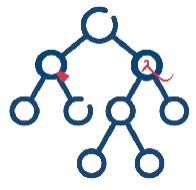
\includegraphics[height=1.0cm]{msca_logo.png}}%
    \end{center}

    \vspace{0.6cm}

    % Main title with Q logos on sides (with clickable links)
    \begin{center}
        \begin{minipage}{0.1\textwidth}
            \centering
            \href{https://quantlet.com}{
\includegraphics[height=1.1cm]{ql_logo.png}}
        \end{minipage}%
        \begin{minipage}{0.78\textwidth}
            \centering
            {\LARGE\bfseries\usebeamercolor[fg]{title}\inserttitle}

            \vspace{0.3cm}

            {\usebeamerfont{subtitle}\usebeamercolor[fg]{title}\insertsubtitle}
        \end{minipage}%
        \begin{minipage}{0.1\textwidth}
            \centering
            \href{https://quantinar.com}{
\includegraphics[height=1.1cm]{qr_logo.png}}
        \end{minipage}
    \end{center}

    \vspace{0.6cm}

    % Authors (left aligned)
    \hspace{0.5cm}{\usebeamerfont{author}\insertauthor}

    \vspace{0.3cm}

    % Institute/Affiliations (left aligned)
    \hspace{0.5cm}\begin{minipage}[t]{0.9\textwidth}
        \raggedright\small\insertinstitute
    \end{minipage}
}

%=============================================================================
% THEOREM ENVIRONMENTS
%=============================================================================
\theoremstyle{definition}
\setbeamertemplate{theorems}[numbered]
\ifdefined\sfmlang
\newtheorem{defn}{Definiție}
\newtheorem{thm}{Teoremă}
\newtheorem{prop}{Propoziție}
\newtheorem{rmk}{Observație}
\else
\newtheorem{defn}{Definition}
\newtheorem{thm}{Theorem}
\newtheorem{prop}{Proposition}
\newtheorem{rmk}{Remark}
\fi

%=============================================================================
% CENTRED MINIPAGE (no extra vertical space)
%=============================================================================
\newenvironment{cminipage}[1]{%
    \par\noindent\hfill\begin{minipage}{#1}\ignorespaces
}{%
    \end{minipage}\hfill\null\par
}

%=============================================================================
% CUSTOM COMMANDS
%=============================================================================
\newcommand{\E}{\mathbb{E}}
\newcommand{\Var}{\text{Var}}
\newcommand{\Cov}{\text{Cov}}
\newcommand{\Corr}{\text{Corr}}
\newcommand{\R}{\mathbb{R}}
\newcommand{\N}{\mathbb{N}}
\newcommand{\Z}{\mathbb{Z}}
\newcommand{\B}{\mathbf{B}}
\newcommand{\imark}{\textcolor{MainBlue}{\textbullet}}
\newcommand{\RMSE}{\text{RMSE}}
\newcommand{\MAE}{\text{MAE}}
\newcommand{\MAPE}{\text{MAPE}}



\newcommand{\qlurl}[1]{https://github.com/danpele/SFM/tree/main/Quantlets/Ch_04/#1}

% Clickable citations (DOIs verified via Crossref)

\newcommand{\refFHH}{\href{https://doi.org/10.1007/978-3-030-13751-9}{Franke, Härdle \& Hafner (2019)}}
\newcommand{\refFHHex}{\href{https://doi.org/10.1007/978-3-642-33929-5}{Borak, Härdle \& López-Cabrera (2013)}}
\newcommand{\refKolmogorov}{\href{https://doi.org/10.1007/978-3-642-49888-6}{Kolmogoroff (1933)}}
\newcommand{\refBachelier}{\href{https://doi.org/10.24033/asens.476}{Bachelier (1900)}}
\newcommand{\refEinstein}{\href{https://doi.org/10.1002/andp.19053220806}{Einstein (1905)}}
\newcommand{\refWiener}{\href{https://doi.org/10.1002/sapm192321131}{Wiener (1923)}}
\newcommand{\refOsborne}{\href{https://doi.org/10.1287/opre.7.2.145}{Osborne (1959)}}
\newcommand{\refBS}{\href{https://doi.org/10.1086/260062}{Black \& Scholes (1973)}}
\newcommand{\refCRR}{\href{https://doi.org/10.1016/0304-405X(79)90015-1}{Cox, Ross \& Rubinstein (1979)}}
\newcommand{\refMU}{\href{https://doi.org/10.1080/01621459.1949.10483310}{Metropolis \& Ulam (1949)}}
\newcommand{\refMarsaglia}{\href{https://doi.org/10.1073/pnas.61.1.25}{Marsaglia (1968)}}
\newcommand{\refMT}{\href{https://doi.org/10.1145/272991.272995}{Matsumoto \& Nishimura (1998)}}
\newcommand{\refGlasserman}{\href{https://doi.org/10.1007/978-0-387-21617-1}{Glasserman (2003)}}
\newcommand{\refEngle}{\href{https://doi.org/10.2307/1912773}{Engle (1982)}}
\newcommand{\refBollerslev}{\href{https://doi.org/10.1016/0304-4076(86)90063-1}{Bollerslev (1986)}}
\newcommand{\refFama}{\href{https://doi.org/10.2307/2325486}{Fama (1970)}}
\newcommand{\refCont}{\href{https://doi.org/10.1080/713665670}{Cont (2001)}}
\newcommand{\refPeleCrypto}{\href{https://doi.org/10.1080/1351847X.2021.1960403}{Pele et al.\ (2023)}}
\newcommand{\refWang}{\href{https://doi.org/10.1038/s41586-023-06221-2}{Wang et al.\ (2023)}}

\title[Statistics of Financial Markets]{Statistics of Financial Markets}
\subtitle{Chapter 4: Probability}
\author[D.T. Pele]{Daniel Traian PELE}
\institute{Bucharest University of Economic Studies\\
IDA Institute Digital Assets\\
Blockchain Research Center\\
AI4EFin Artificial Intelligence for Energy Finance\\
Romanian Academy, Institute for Economic Forecasting\\
MSCA Digital Finance}
\date{}

%=============================================================================
\providecommand{\sfmapplink}[3]{\hypertarget{#2}{}\hyperlink{#1}{\beamergotobutton{#3}}}  % APPLINKS-MACROS
\providecommand{\sfmappback}[2]{\begin{tikzpicture}[remember picture,overlay]\node[anchor=south east] at ([xshift=-3mm,yshift=7mm]current page.south east){\hyperlink{#1}{\beamerreturnbutton{#2}}};\end{tikzpicture}}  % APPLINKS-MACROS
\providecommand{\sfmchlink}[2]{\href{#1}{#2}}  % APPLINKS-MACROS
\providecommand{\sfmchlinkt}[2]{\href{#1}{\usebeamercolor[fg]{frametitle}#2}}  % APPLINKS-MACROS
\begin{document}
%=============================================================================

{
\setbeamertemplate{headline}{}
\setbeamertemplate{footline}{}
\begin{frame}[noframenumbering]
    \titlepage
\end{frame}
}
% BEGIN-ACRONYMS (generat de latex/acronyms.py; nu editati manual)
\begin{frame}{Acronyms used in this material}
\setbeamertemplate{itemize/enumerate body begin}{\tiny}
\begin{columns}[T]
\begin{column}{0.49\textwidth}
\begin{itemize}\setlength{\itemsep}{0pt}
    \item \textbf{AI}: Artificial Intelligence
    \item \textbf{AR}: AutoRegressive (model)
    \item \textbf{ARCH}: AutoRegressive Conditional Heteroskedasticity
    \item \textbf{BET}: Bucharest Exchange Trading (index)
    \item \textbf{CDF}: Cumulative Distribution Function
    \item \textbf{CLT}: Central Limit Theorem
    \item \textbf{CRR}: Cox–Ross–Rubinstein (binomial model)
    \item \textbf{ES}: Expected Shortfall
    \item \textbf{GARCH}: Generalised AutoRegressive Conditional Heteroskedasticity
    \item \textbf{GBM}: Geometric Brownian Motion
    \item \textbf{IBM}: International Business Machines (company)
    \item \textbf{LCG}: Linear Congruential Generator
    \item \textbf{LLN}: Law of Large Numbers
\end{itemize}
\end{column}
\begin{column}{0.49\textwidth}
\begin{itemize}\setlength{\itemsep}{0pt}
    \item \textbf{PCG64}: Permuted Congruential Generator, 64-bit (NumPy default)
    \item \textbf{PMF}: Probability Mass Function
    \item \textbf{RANDU}: RANDU (IBM random number generator of the 1960s)
    \item \textbf{SFE}: Statistics of Financial Markets, Exercises (Quantlet collection of the textbook)
\end{itemize}
\end{column}
\end{columns}
\end{frame}
% END-ACRONYMS

\begin{frame}{Today's Question and Route}
\itemsize{\small}
\begin{itemize}
    \item \textbf{Question}: which probability tools do we need to describe returns and to simulate prices?
    \begin{itemize}
        \item every later chapter (tails, volatility, VaR, efficiency) is built on them
    \end{itemize}
    \item \textbf{Route} of the chapter
    \begin{itemize}
        \item random variables, distributions, expectation, variance, covariance
        \item independence vs uncorrelatedness, conditional expectation and conditional variance
        \item random numbers and Monte Carlo; the binomial model
        \item random walk, martingale, white noise, AR(1); Wiener process and GBM
    \end{itemize}
    \item Real data, 2000--2026: S\&P 500, DAX, BET and Bitcoin (from 2014)
\end{itemize}
\end{frame}

\begin{frame}{Learning Outcomes}
\itemsize{\small}
\begin{itemize}
    \item Compute expectations, variances, covariances and correlations, and the volatility of a portfolio
    \item Explain why uncorrelated returns can still be dependent, and measure it
    \item Use conditional expectation and conditional variance, the building blocks of GARCH
    \item Generate random numbers with the inverse transform and estimate a probability by Monte Carlo, with its standard error
    \item Define a random walk, a martingale, white noise, the Wiener process and GBM, and simulate them
\end{itemize}
\end{frame}

\begin{frame}{Reading and Tools}
\itemsize{\small}
\begin{itemize}
    \item Textbook: \refFHH, \textit{Statistics of Financial Markets}, 5th ed., Ch.~3 (Sec.~3.1--3.5) and Ch.~4 (discrete-time stochastic processes)
    \begin{itemize}
        \item exercises with solutions: \refFHHex, Ch.~3--4
    \end{itemize}
    \item Monte Carlo methods in finance: \refGlasserman
    \item Python Quantlets of this chapter: \href{https://github.com/danpele/SFM/tree/main/Quantlets/Ch_04}{Quantlets/Ch\_04}
    \begin{itemize}
        \item ported from the SFE Quantlets of the textbook (SFErandu, SFErangen1, SFErangen2, SFEBinomp, SFEWienerProcess, SFEsimGBM)
        \item each chart in these slides links to the Quantlet that draws it
    \end{itemize}
    \item Lecture notebook: \href{\colaburl{notebooks/EN/chapter4_lecture_notebook.ipynb}}{open in Google Colab}
    \item Video course: \quantinar{Statistics of Financial Markets}{https://quantinar.com/course/103/statistics-of-financial-markets}
\end{itemize}
\end{frame}


%=============================================================================
\section{From Games of Chance to Axioms}
%=============================================================================

\begin{frame}{1654: the Problem of Points}
\itemsize{\small}
\begin{columns}[T]
\begin{column}{0.60\textwidth}
\begin{itemize}
    \item Two players stop a fair game before the end: how should the stake be split?
    \item Blaise Pascal and Pierre de Fermat solved it in letters (1654): split by the probability of winning, not by the score
    \item Example: A needs 1 more win, B needs 2; at most two more rounds
    \begin{itemize}
        \item B wins only if B wins both rounds: probability $1/4$
        \item A should get 75\% of the stake: its \textbf{expected} gain
    \end{itemize}
    \item The same idea prices a derivative today: a fair price is an expected payoff
\end{itemize}
\end{column}
\begin{column}{0.36\textwidth}
\centering
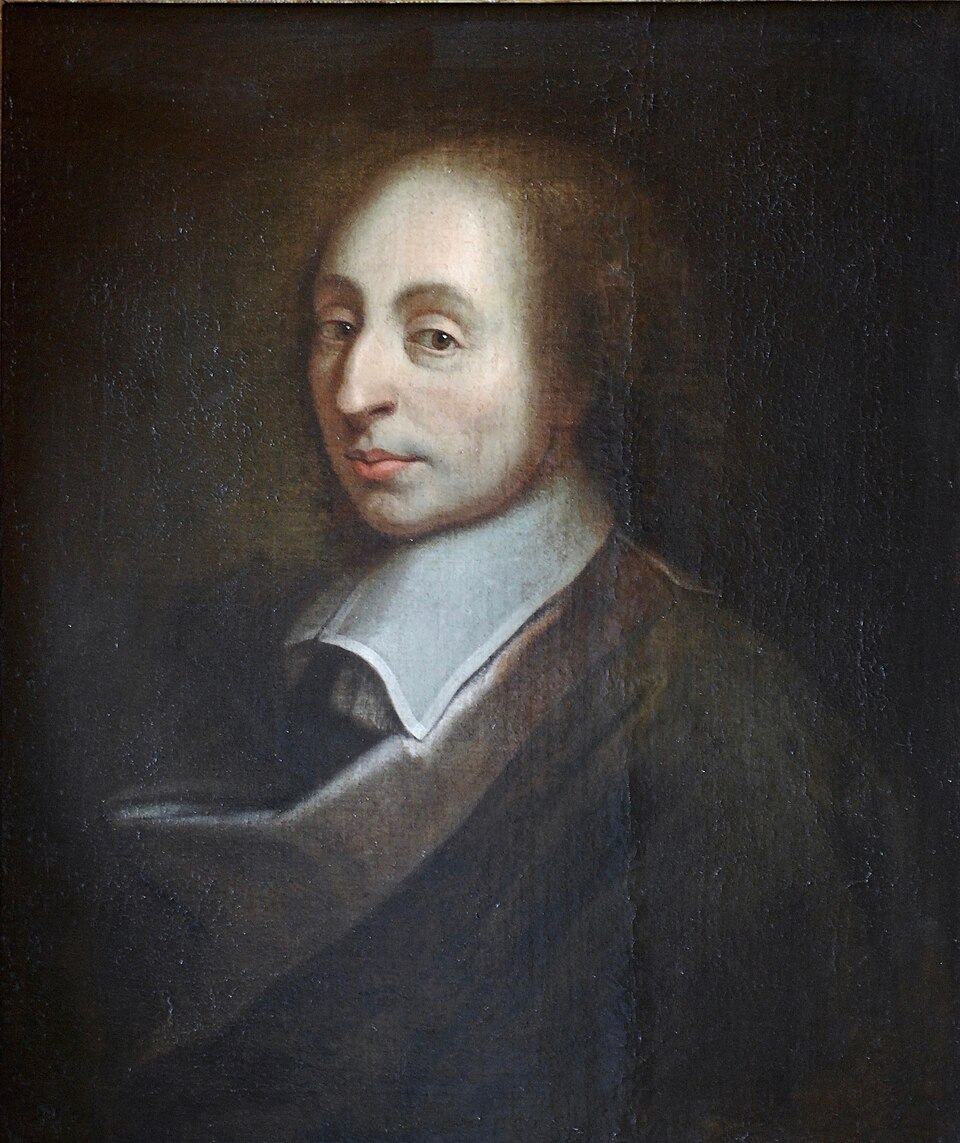
\includegraphics[height=0.55\textheight]{ch4_pascal.jpg}\\[1mm]
\imgcap{Blaise Pascal (1623--1662)}
\imgcredit{https://commons.wikimedia.org/wiki/File:Blaise_Pascal_Versailles.JPG}{Portrait: unknown author, after François II Quesnel (c. 1690); public domain; Wikimedia Commons}
\end{column}
\end{columns}
\end{frame}

\begin{frame}{Kolmogorov's Axioms (1933)}
\itemsize{\footnotesize}
\begin{columns}[T]
\begin{column}{0.62\textwidth}
\begin{itemize}
    \item A \textbf{probability space} $(\Omega, \mathcal{F}, P)$ \refKolmogorov
    \begin{itemize}
        \item $\Omega$: all possible outcomes (all possible paths of tomorrow's market)
        \item $\mathcal{F}$: the events we can assign a probability to (a $\sigma$-algebra)
        \item $P$: a function from events to $[0, 1]$
    \end{itemize}
    \item Axioms, for any event $A \in \mathcal{F}$
    \begin{itemize}
        \item $P(A) \ge 0$: no probability is negative
        \item $P(\Omega) = 1$: some outcome certainly occurs
        \item $P(\cup_i A_i) = \sum_i P(A_i)$ for disjoint $A_1, A_2, \dots$ (no two can occur together): the probability of ``one of them'' is the sum
    \end{itemize}
    \item Everything else (expectation, independence, processes) is built on these three rules
\end{itemize}
\end{column}
\begin{column}{0.34\textwidth}
\centering
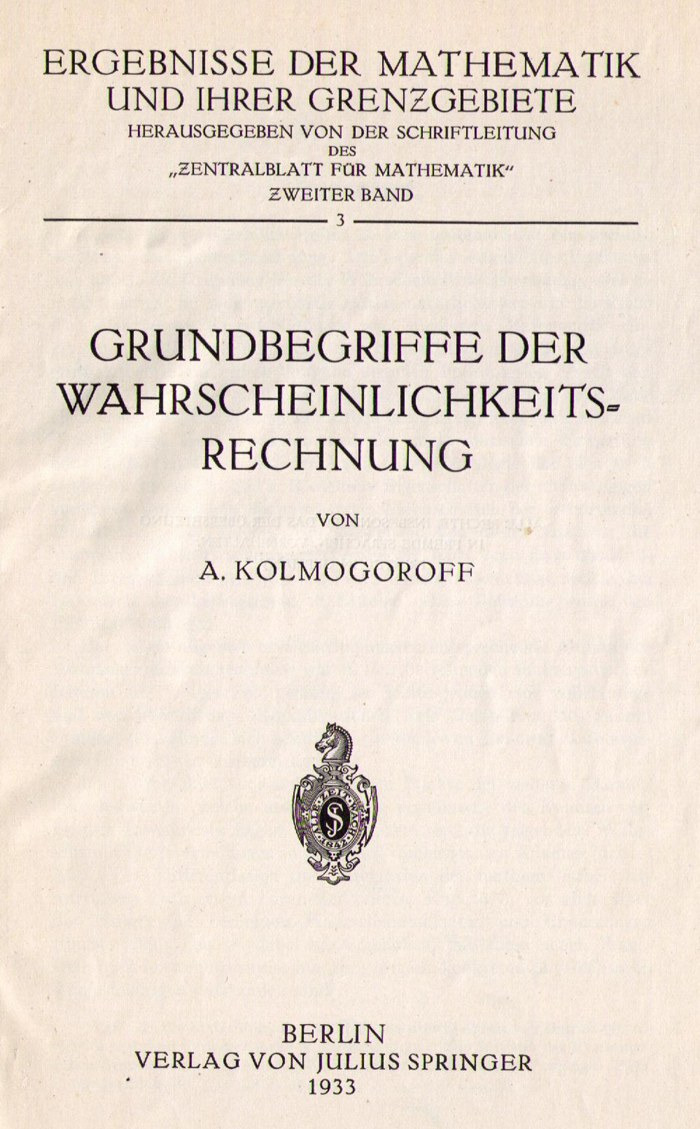
\includegraphics[height=0.56\textheight]{ch4_kolmogorov_grundbegriffe.jpg}\\[1mm]
\imgcap{Title page of the \textit{Grundbegriffe}, Springer 1933}
\imgcredit{https://commons.wikimedia.org/wiki/File:Kolmogoroff_Grundbegriffe.png}{Photo: KurtSchwitters (2012); CC BY-SA 3.0; Wikimedia Commons}
\end{column}
\end{columns}
\end{frame}

\begin{frame}{Andrey Kolmogorov}
\itemsize{\small}
\begin{columns}[T]
\begin{column}{0.44\textwidth}
\begin{itemize}
    \item Andrey Nikolaevich Kolmogorov (1903--1987), Moscow State University
    \item Made probability a branch of measure theory: events are sets, probability is a measure
    \item Also: conditional expectation in its modern form, Markov processes, turbulence, complexity
    \item The Kolmogorov--Smirnov test (\sfmchlink{https://danpele.github.io/SFM/EN/Courses/chapter6_model_selection_risk_management.pdf}{Chapter 6}) carries his name
\end{itemize}
\end{column}
\begin{column}{0.52\textwidth}
\centering
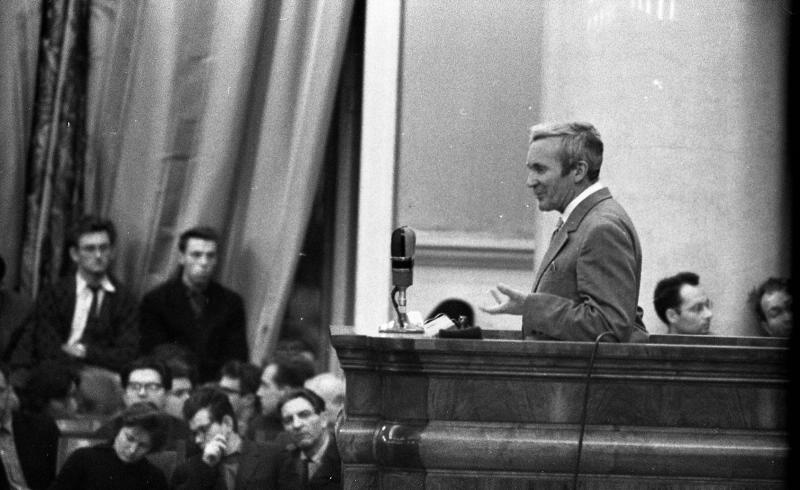
\includegraphics[height=0.40\textheight]{ch4_kolmogorov_1963.jpg}\\[1mm]
\imgcap{Kolmogorov lecturing in Moscow, 1963--1964}
\imgcredit{https://commons.wikimedia.org/wiki/File:\%D0\%9C\%D0\%B0\%D1\%82\%D0\%B5\%D0\%BC\%D0\%B0\%D1\%82\%D0\%B8\%D0\%BA_\%D0\%90\%D0\%BD\%D0\%B4\%D1\%80\%D0\%B5\%D0\%B9_\%D0\%9A\%D0\%BE\%D0\%BB\%D0\%BC\%D0\%BE\%D0\%B3\%D0\%BE\%D1\%80\%D0\%BE\%D0\%B2_\%D0\%B2_\%D0\%B0\%D1\%83\%D0\%B4\%D0\%B8\%D1\%82\%D0\%BE\%D1\%80\%D0\%B8\%D0\%B8.jpg}{Photo: Vsevolod Tarasevich (1963--1964); CC BY 4.0; Wikimedia Commons}
\end{column}
\end{columns}
\end{frame}

\begin{frame}{Events, Conditional Probability, Independence}
\itemsize{\footnotesize}
\begin{itemize}
    \item \textbf{Conditional probability}: $P(A \mid B) = P(A \cap B)/P(B)$, for $P(B) > 0$
    \begin{itemize}
        \item $A, B$: two events; $A \cap B$: both occur
        \item in words: among the cases in which $B$ occurs, the share in which $A$ also occurs
    \end{itemize}
    \item \textbf{Bayes' rule}: $P(B \mid A) = P(A \mid B)P(B)/P(A)$
    \begin{itemize}
        \item $P(B)$: the probability of $B$ before we learn $A$; $P(B \mid A)$: the updated probability once $A$ is observed
        \item it reverses the direction of conditioning: from ``signal given crisis'' to ``crisis given signal''
    \end{itemize}
    \item \textbf{Independent} events: $P(A \cap B) = P(A)P(B)$, i.e. $P(A \mid B) = P(A)$
    \begin{itemize}
        \item learning that $B$ occurred does not change the probability of $A$
    \end{itemize}
\end{itemize}
\end{frame}

\begin{frame}{Example: Down Days in a Row}
\itemsize{\small}
\begin{itemize}
    \item S\&P 500, 2000--2026: $P(\text{down day}) = 46.3\%$
    \begin{itemize}
        \item after a down day: $P(\text{down} \mid \text{down yesterday}) = 43.4\%$
        \item two down days in a row: 20.1\% in the data
        \item under independence: $P(\text{down})^2 = 21.4\%$, close to the data
    \end{itemize}
    \item BET: 50.0\% after a down day vs 42.6\% after an up day
    \begin{itemize}
        \item the sign of the return persists from one day to the next
        \item a consequence of thin trading: prices adjust to news over several days
    \end{itemize}
\end{itemize}
\end{frame}

\begin{frame}{Recap: From Games to Axioms}
\itemsize{\small}
\begin{itemize}
    \item Probability space $(\Omega, \mathcal{F}, P)$ and three axioms
    \item Fair value = expected value: the idea of Pascal and Fermat
    \item Conditional probability measures how information changes the odds
\end{itemize}
\end{frame}


%=============================================================================
\section{Random Variables and Distributions}
%=============================================================================

\begin{frame}{Random Variables}
\itemsize{\footnotesize}
\begin{itemize}
    \item A \textbf{random variable} $X: \Omega \to \mathbb{R}$ assigns a number to each outcome
    \begin{itemize}
        \item tomorrow's log return, the number of up days in a week, the loss of a portfolio
    \end{itemize}
    \item \textbf{Discrete}: finitely or countably many values $x_i$
    \begin{itemize}
        \item \textbf{PMF} (probability mass function): $p(x_i) = P(X = x_i)$, with $\sum_i p(x_i) = 1$
        \item $p(x_i)$: the probability of the value $x_i$; the probabilities of all values add up to 1
    \end{itemize}
    \item \textbf{Continuous}: $P(a < X \le b) = \int_a^b f(x)\,dx$
    \begin{itemize}
        \item the probability of an interval $(a, b]$ is the area under $f$ between $a$ and $b$
        \item $f$ is the \textbf{PDF} (probability density function): $f \ge 0$ and the total area $\int f = 1$
        \item a single point has no area: $P(X = x) = 0$ for every $x$
    \end{itemize}
    \item Textbook: \refFHH, Sec.~3.1
\end{itemize}
\end{frame}

\begin{frame}{The Distribution Function and the Quantile Function}
\itemsize{\small}
\begin{itemize}
    \item \textbf{CDF} (cumulative distribution function): $F(x) = P(X \le x)$
    \begin{itemize}
        \item the probability that $X$ does not exceed the threshold $x$
        \item non-decreasing, right-continuous, from $F(-\infty) = 0$ to $F(\infty) = 1$
        \item for a continuous $X$ the density is its derivative: $f = F'$
    \end{itemize}
    \item \textbf{Quantile} of order $\alpha$: $q_\alpha = F^{-1}(\alpha) = \inf\{x : F(x) \ge \alpha\}$
    \begin{itemize}
        \item $\alpha \in (0, 1)$: a probability; $q_\alpha$ is the smallest $x$ with $P(X \le x) \ge \alpha$
        \item $F^{-1}$: the quantile function, the inverse of the CDF; $\inf$: the smallest value of the set
        \item median $= q_{0.5}$; the 1\% quantile is the return exceeded on 99\% of the days
    \end{itemize}
\end{itemize}
\end{frame}

\begin{frame}{Value at Risk and the Empirical CDF}
\itemsize{\small}
\begin{itemize}
    \item \textbf{VaR} (Value at Risk) 1\%: $\text{VaR}_{1\%} = -q_{0.01}$
    \begin{itemize}
        \item $q_{0.01}$: the 1\% quantile of the returns, a negative number
        \item the minus sign turns it into a loss: the loss exceeded with probability 1\%
        \item estimation and backtesting in \sfmchlink{https://danpele.github.io/SFM/EN/Courses/chapter10_var_es_backtesting.pdf}{Chapter 10}
    \end{itemize}
    \item The \textbf{empirical CDF} of a sample: $\hat F(x) = \frac1n \#\{t : r_t \le x\}$
    \begin{itemize}
        \item $r_1, \dots, r_n$: the observed returns; $n$: the sample size
        \item $\#\{\cdot\}$: the number of days in the set; $\hat F(x)$ is the share of days with a return at most $x$
        \item the hat marks an estimate computed from data
    \end{itemize}
\end{itemize}
\end{frame}

\begin{frame}{A Discrete and a Continuous Random Variable}
\itemsize{\footnotesize}
\begin{center}
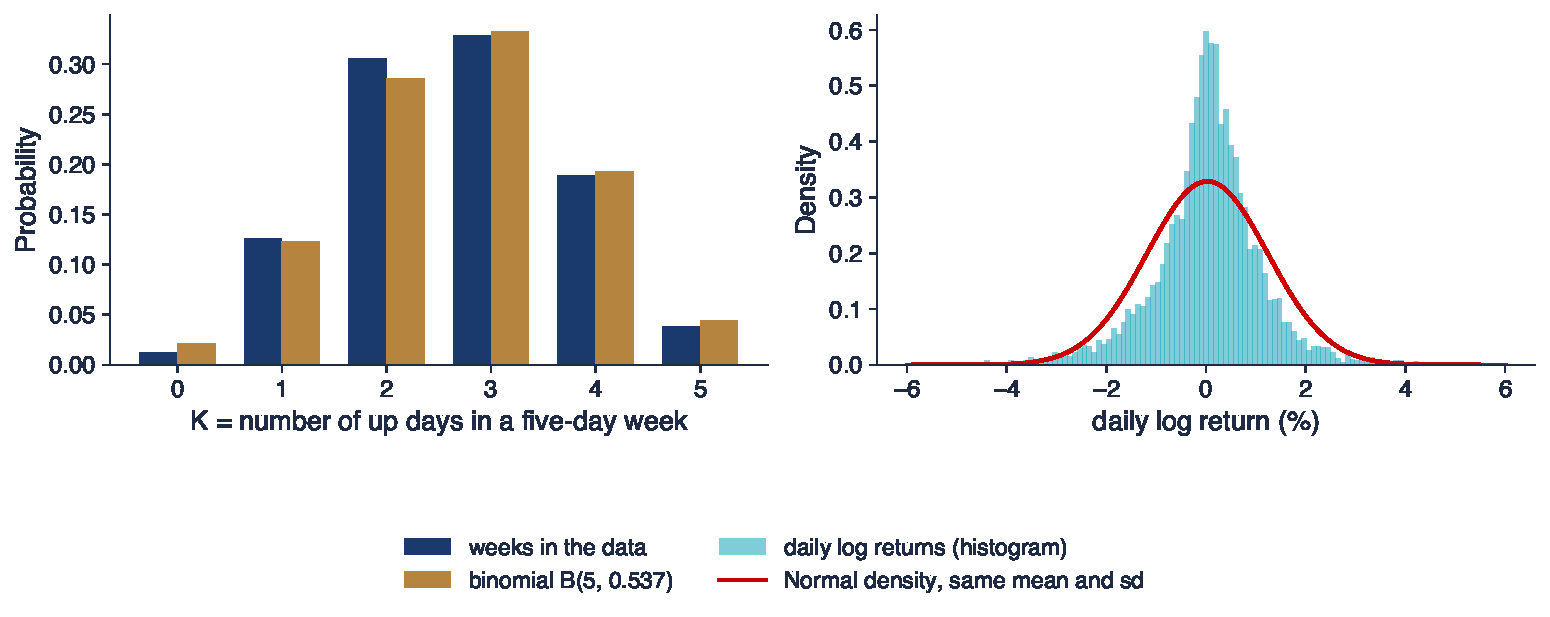
\includegraphics[width=0.97\textwidth,height=0.56\textheight,keepaspectratio]{sfm_ch4_random_variables.pdf}
\end{center}
\vspace{-0.25cm}
\begin{itemize}
    \item Left: $K$ = number of up days in a full week of the S\&P 500 (1\,144 weeks)
    \begin{itemize}
        \item compared with $B(5, p)$, the binomial distribution: 5 days, each up with probability $p = 0.537$
        \item mean 2.67 vs 2.69; variance 1.16 vs 1.24
    \end{itemize}
    \item Right: daily log returns, a continuous random variable; the histogram estimates the PDF
    \item The binomial fits $K$ well; the Normal density misses the peak and the tails of the returns (\sfmchlink{https://danpele.github.io/SFM/EN/Courses/chapter2_classical_distributions_stylised_facts.pdf}{Chapter 2})
\end{itemize}
\sfmquantlet{Ch_04}{SFM_ch4_random_variables}
\end{frame}

\begin{frame}{Empirical CDF and the 1\% Quantile of the S\&P 500}
\itemsize{\footnotesize}
\begin{center}
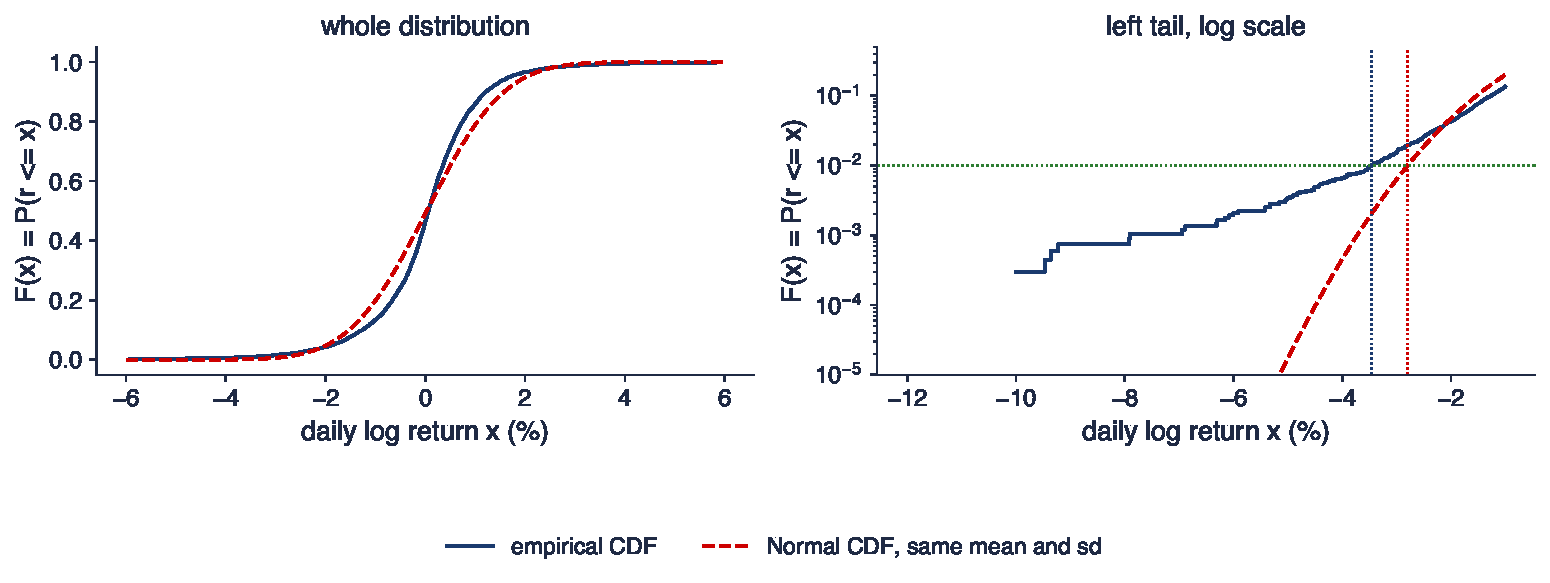
\includegraphics[width=0.97\textwidth,height=0.56\textheight,keepaspectratio]{sfm_ch4_cdf_quantile.pdf}
\end{center}
\vspace{-0.25cm}
\begin{itemize}
    \item $n = 6\,714$ days; median $0.063\%$; $\hat F(0) = 46.3\%$ of the days are not up days
    \item VaR 1\%: empirical 3.45\%, Normal 2.80\%; $P(r < -3\%)$: 1.55\% vs 0.63\%
    \item $P(r < -5\%)$: 0.34\% in the data, 199 times the value under the Normal distribution ($1.7 \times 10^{-3}\%$)
\end{itemize}
\sfmquantlet{Ch_04}{SFM_ch4_random_variables}
\end{frame}

\begin{frame}{Recap: Random Variables}
\itemsize{\small}
\begin{itemize}
    \item PMF for discrete, PDF for continuous variables; the CDF works for both
    \item Quantiles invert the CDF; VaR 1\% is minus the 1\% quantile
    \item The tails of the empirical CDF are much heavier than the Normal ones
\end{itemize}
\end{frame}


%=============================================================================
\section{Expectation and Variance}
%=============================================================================

\begin{frame}{Expectation}
\itemsize{\footnotesize}
\begin{itemize}
    \item \textbf{Expectation} (mean): $E[X] = \sum_i x_i p(x_i)$ or $E[X] = \int x f(x)\,dx$
    \begin{itemize}
        \item $x_i$, $p(x_i)$: the values and their probabilities; $f$: the density
        \item the centre of mass of the distribution; it exists only if $E|X| < \infty$ (not for Cauchy, \sfmchlink{https://danpele.github.io/SFM/EN/Courses/chapter3_alpha_stable_distributions.pdf}{Chapter 3})
    \end{itemize}
    \item Of a function: $E[g(X)] = \int g(x) f(x)\,dx$, without finding the distribution of $g(X)$
    \item \textbf{Linearity}: $E[aX + bY + c] = aE[X] + bE[Y] + c$, always (no independence needed)
    \begin{itemize}
        \item $a, b, c$: constants; $X, Y$: any two random variables
        \item the expected return of a portfolio is the weighted mean of the expected returns
    \end{itemize}
    \item In general $E[g(X)] \ne g(E[X])$
    \begin{itemize}
        \item Jensen: for a convex $g$, $E[g(X)] \ge g(E[X])$; for example $E[e^X] > e^{E[X]}$
        \item the source of the volatility drag of \sfmchlink{https://danpele.github.io/SFM/EN/Courses/chapter1_data_returns_indicators.pdf}{Chapter 1}
    \end{itemize}
\end{itemize}
\end{frame}

\begin{frame}{Variance and Moments}
\itemsize{\small}
\begin{itemize}
    \item \textbf{Variance}: $\text{Var}(X) = E[(X - \mu)^2] = E[X^2] - \mu^2$
    \begin{itemize}
        \item $\mu = E[X]$; the variance is the mean squared distance from the mean
        \item standard deviation $\sigma = \sqrt{\text{Var}(X)}$, in the units of $X$; for returns it is the volatility
    \end{itemize}
    \item $\text{Var}(aX + b) = a^2\,\text{Var}(X)$
    \begin{itemize}
        \item adding a constant $b$ does not change risk; multiplying by $a$ multiplies the variance by $a^2$
    \end{itemize}
    \item Moments: $E[X^k]$ for $k = 1, 2, \dots$
    \begin{itemize}
        \item skewness and kurtosis use $k = 3, 4$ (\sfmchlink{https://danpele.github.io/SFM/EN/Courses/chapter2_classical_distributions_stylised_facts.pdf}{Chapter 2})
    \end{itemize}
\end{itemize}
\end{frame}

\begin{frame}{Worked Example: Annual Mean and Volatility}
\itemsize{\small}
\begin{itemize}
    \item S\&P 500, daily log returns $r_t$
    \begin{itemize}
        \item daily mean $0.0247\%$, daily standard deviation $\sigma = 1.213\%$
        \item $A = 251$: the number of trading days per year
    \end{itemize}
    \item Assume i.i.d. daily returns (independent and identically distributed)
    \begin{itemize}
        \item the annual log return is the sum of the $A$ daily ones: $\sum_{t=1}^{A} r_t$
    \end{itemize}
    \item Mean: $E[\sum r_t] = A \times 0.0247 = 6.2\%$ a year
    \begin{itemize}
        \item linearity of expectation
    \end{itemize}
    \item Variance: $\text{Var}(\sum r_t) = A\,\sigma^2$, because the covariances are zero
    \begin{itemize}
        \item annual volatility $\sigma\sqrt{A} = 1.213\sqrt{251} = 19.2\%$
        \item the square-root-of-time rule: volatility grows with $\sqrt{h}$ over $h$ periods
    \end{itemize}
\end{itemize}
\end{frame}

\begin{frame}{How Rare Is a 4-Sigma Day? Chebyshev's Bound}
\itemsize{\small}
\begin{itemize}
    \item \textbf{Chebyshev's inequality}: for any $X$ with finite variance, $P(|X - \mu| \ge k\sigma) \le 1/k^2$
    \begin{itemize}
        \item $\mu$, $\sigma$: the mean and the standard deviation; $k > 1$: the distance from the mean, in standard deviations
        \item it uses only the mean and the variance, so it holds for every distribution
    \end{itemize}
    \item $k = 4$, S\&P 500, 2000--2026
    \begin{itemize}
        \item Chebyshev bound: at most 6.25\% of the days
        \item Normal distribution: 0.0063\%
        \item data: 46 days, 0.69\%
    \end{itemize}
    \item The data lie between the two
    \begin{itemize}
        \item the Normal distribution is far too optimistic; the worst case of Chebyshev is too pessimistic
    \end{itemize}
\end{itemize}
\end{frame}

\begin{frame}{Recap: Expectation and Variance}
\itemsize{\small}
\begin{itemize}
    \item Expectation is linear; variance scales with the square
    \item For i.i.d. returns the mean grows with $h$ and the volatility with $\sqrt{h}$
    \item Chebyshev bounds tail probabilities for any distribution
\end{itemize}
\end{frame}


%=============================================================================
\section{Joint Distributions and Dependence}
%=============================================================================

\begin{frame}{Joint Distribution and Marginals}
\itemsize{\small}
\begin{itemize}
    \item \textbf{Joint CDF}: $F(x, y) = P(X \le x, Y \le y)$
    \begin{itemize}
        \item the probability that both variables are below their thresholds at the same time
        \item for two returns: both markets fall below given levels on the same day
    \end{itemize}
    \item \textbf{Marginal} CDF: $F_X(x) = F(x, \infty)$
    \begin{itemize}
        \item the distribution of $X$ alone, whatever the value of $Y$
    \end{itemize}
    \item \textbf{Joint PDF} $f(x, y)$: $P((X, Y) \in B) = \iint_B f(x, y)\,dx\,dy$
    \begin{itemize}
        \item $B$: a region of the plane; the probability is the volume under $f$ above $B$
        \item marginal density: $f_X(x) = \int f(x, y)\,dy$, integrating $Y$ out
    \end{itemize}
\end{itemize}
\end{frame}

\begin{frame}{Covariance, Correlation and the Variance of a Sum}
\itemsize{\footnotesize}
\begin{itemize}
    \item \textbf{Covariance}: $\text{Cov}(X, Y) = E[(X - \mu_X)(Y - \mu_Y)] = E[XY] - \mu_X\mu_Y$
    \begin{itemize}
        \item $\mu_X$, $\mu_Y$: the means; positive when $X$ and $Y$ tend to be above their means together
    \end{itemize}
    \item \textbf{Correlation}: $\rho = \text{Cov}(X, Y)/(\sigma_X\sigma_Y) \in [-1, 1]$
    \begin{itemize}
        \item the covariance divided by the two standard deviations: a number without units
        \item measures \textbf{linear} dependence only; $|\rho| = 1$ iff $Y = a + bX$
    \end{itemize}
    \item \textbf{Variance of a sum}: $\text{Var}(aX + bY) = a^2\sigma_X^2 + b^2\sigma_Y^2 + 2ab\,\text{Cov}(X, Y)$
    \begin{itemize}
        \item $a, b$: constants (in a portfolio, the weights); the covariance term can raise or lower the risk
        \item many assets: $\sigma_p^2 = w^\top \Sigma w$, with $w$ the vector of weights and $\Sigma$ the covariance matrix
        \item $\sigma_p^2$: the variance of the portfolio; $w^\top$: the transposed vector
    \end{itemize}
\end{itemize}
\end{frame}

\begin{frame}{Joint Distributions of Daily Returns}
\itemsize{\footnotesize}
\begin{center}
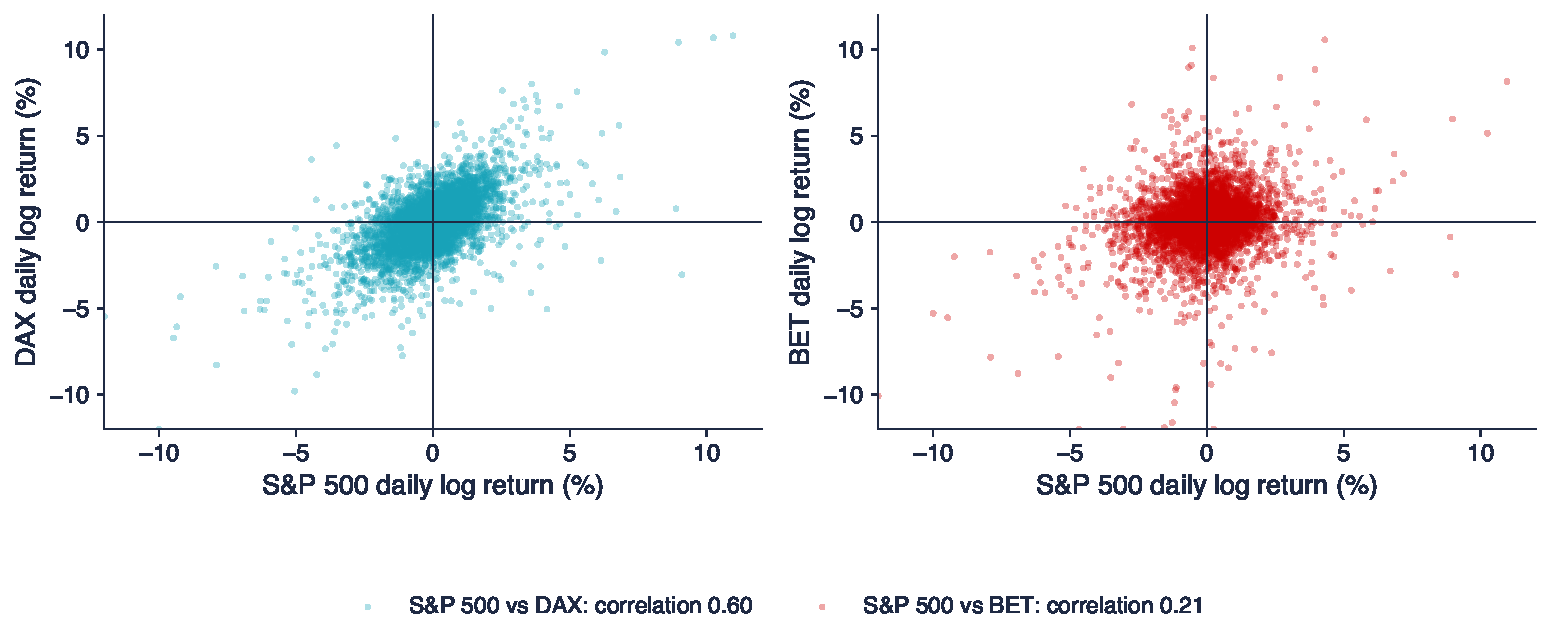
\includegraphics[width=0.97\textwidth,height=0.56\textheight,keepaspectratio]{sfm_ch4_joint.pdf}
\end{center}
\vspace{-0.25cm}
\begin{itemize}
    \item Common trading days only: prices are joined first, then differenced ($n = 6\,605$ days for S\&P 500 and DAX)
    \item S\&P 500 and DAX: $\rho = 0.60$; S\&P 500 and BET: $\rho = 0.21$
    \item The cloud is elliptic in the centre, but extreme days are joint: crises hit all markets together
\end{itemize}
\sfmquantlet{Ch_04}{SFM_ch4_dependence}
\end{frame}

\begin{frame}{Worked Example: a 50/50 Portfolio of S\&P 500 and DAX}
\itemsize{\footnotesize}
\begin{itemize}
    \item Daily standard deviations: $\sigma_1 = 1.22\%$ (S\&P 500), $\sigma_2 = 1.43\%$ (DAX)
    \begin{itemize}
        \item covariance $1.045$; correlation $0.60$
        \item weights $a = b = 0.5$, so $a^2 = b^2 = 0.25$ and $2ab = 0.5$
    \end{itemize}
    \item $\sigma_p^2 = 0.25\sigma_1^2 + 0.25\sigma_2^2 + 2 \times 0.25\,\text{Cov} = 0.883 + 0.522 = 1.405$
    \begin{itemize}
        \item $\sigma_p = 1.19\%$, below the average volatility $1.32\%$: diversification
    \end{itemize}
    \item S\&P 500 and BET, lower correlation: $\sigma_p = 1.04\%$ vs average $1.33\%$
    \begin{itemize}
        \item the lower the correlation, the larger the reduction in risk
    \end{itemize}
    \item Diversification works only through $\rho < 1$
    \begin{itemize}
        \item in a crash correlations rise, exactly when diversification is needed
    \end{itemize}
\end{itemize}
\end{frame}

\begin{frame}{Independence and Uncorrelatedness}
\itemsize{\small}
\begin{itemize}
    \item $X$ and $Y$ are \textbf{independent} if $F(x, y) = F_X(x)F_Y(y)$ for all $x, y$
    \begin{itemize}
        \item the joint CDF is the product of the marginal CDFs
        \item then $E[g(X)h(Y)] = E[g(X)]E[h(Y)]$ for \textbf{all} functions $g, h$ (for example squares or absolute values)
    \end{itemize}
    \item Independent $\Rightarrow$ uncorrelated ($g, h$ = identity); the converse is false
    \item Example: $X \sim N(0, 1)$, $Y = X^2$
    \begin{itemize}
        \item $\text{Cov}(X, X^2) = E[X^3] = 0$: uncorrelated
        \item but $Y$ is a function of $X$: completely dependent
    \end{itemize}
    \item Exception: for jointly Normal variables, uncorrelated $\Leftrightarrow$ independent
\end{itemize}
\end{frame}

\begin{frame}{Returns Are Uncorrelated, Squared Returns Are Not}
\itemsize{\scriptsize}
\begin{center}
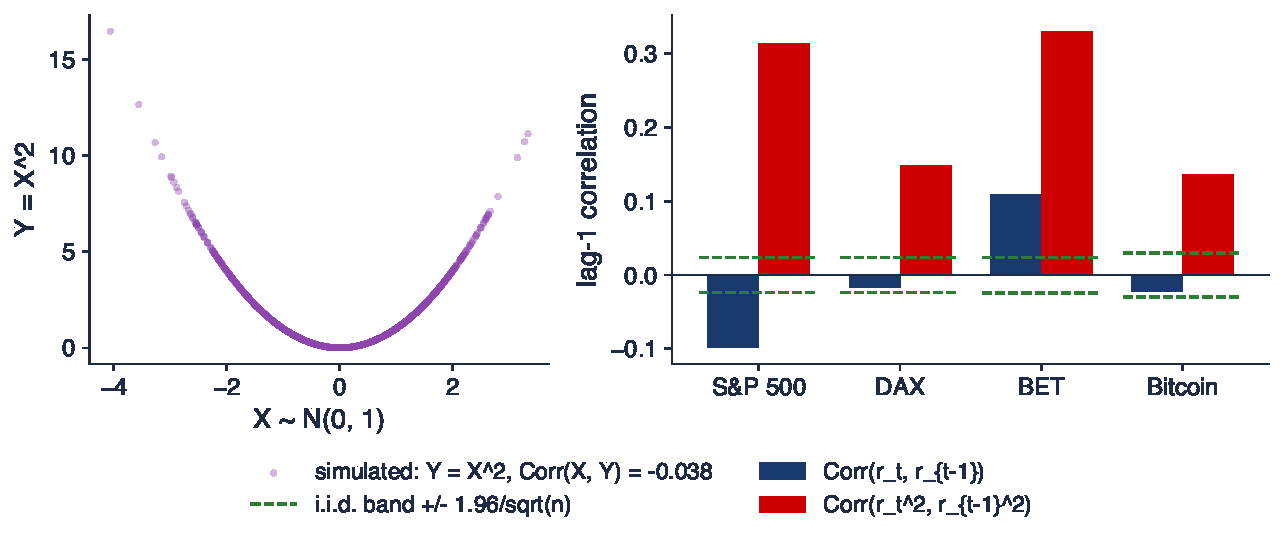
\includegraphics[width=0.97\textwidth,height=0.46\textheight,keepaspectratio]{sfm_ch4_uncorrelated_dependent.pdf}
\end{center}
\vspace{-0.25cm}
\begin{itemize}
    \item Left: simulated $Y = X^2$, sample correlation $-0.038$, yet $Y$ is determined by $X$
    \item Right: $\text{Corr}(r_t, r_{t-1})$ is small: S\&P 500 $-0.099$, DAX $-0.017$, Bitcoin $-0.022$
    \begin{itemize}
        \item $\text{Corr}(r_t^2, r_{t-1}^2)$ is far outside the band: $0.31$, $0.15$, $0.14$
        \item band $\pm 1.96/\sqrt{n}$: the values compatible with zero correlation at the 5\% level
    \end{itemize}
    \item BET: $\text{Corr}(r_t, r_{t-1}) = 0.109$, an effect of thin trading
    \begin{itemize}
        \item the negative S\&P 500 value comes mostly from crisis days
    \end{itemize}
\end{itemize}
\sfmquantlet{Ch_04}{SFM_ch4_dependence}
\end{frame}

\begin{frame}{Recap: Joint Distributions}
\itemsize{\small}
\begin{itemize}
    \item Covariance enters the variance of every portfolio
    \item Independent implies uncorrelated, not the other way round
    \item Returns: nearly uncorrelated, but their squares are correlated, so they are not independent
\end{itemize}
\end{frame}


%=============================================================================
\section{Conditional Expectation and Conditional Variance}
%=============================================================================

\begin{frame}{Conditional Expectation}
\itemsize{\footnotesize}
\begin{itemize}
    \item Conditional density: $f(y \mid x) = f(x, y)/f_X(x)$
    \begin{itemize}
        \item the distribution of $Y$ once we know that $X = x$: the joint density rescaled by the marginal one
    \end{itemize}
    \item \textbf{Conditional expectation}: $E[Y \mid X = x] = \int y f(y \mid x)\,dy$
    \begin{itemize}
        \item the mean of $Y$ computed with the conditional density
        \item $E[Y \mid X]$ is a random variable, a function of $X$
    \end{itemize}
    \item It is the best forecast of $Y$ from $X$: it minimises $E[(Y - g(X))^2]$ over all functions $g$
    \begin{itemize}
        \item $E[(Y - g(X))^2]$: the mean squared error of the forecast $g(X)$
        \item for returns: $E[r_t \mid \mathcal{F}_{t-1}]$, the forecast given all information $\mathcal{F}_{t-1}$ up to yesterday
    \end{itemize}
    \item \textbf{Tower property} (law of iterated expectations): $E\big[E[Y \mid X]\big] = E[Y]$
    \begin{itemize}
        \item averaging the conditional forecasts over all values of $X$ gives back the unconditional mean
    \end{itemize}
\end{itemize}
\end{frame}

\begin{frame}{Conditional Variance and the Law of Total Variance}
\itemsize{\small}
\begin{itemize}
    \item \textbf{Conditional variance}: $\text{Var}(Y \mid X) = E\big[(Y - E[Y \mid X])^2 \mid X\big]$
    \begin{itemize}
        \item the spread of $Y$ around its conditional mean, once $X$ is known
    \end{itemize}
    \item \textbf{Law of total variance}: $\text{Var}(Y) = E\big[\text{Var}(Y \mid X)\big] + \text{Var}\big(E[Y \mid X]\big)$
    \begin{itemize}
        \item $E[\text{Var}(Y \mid X)]$: the average variance inside the groups defined by $X$ (within)
        \item $\text{Var}(E[Y \mid X])$: how much the group means differ from each other (between)
        \item total risk = within-group variance + between-group variance
    \end{itemize}
\end{itemize}
\end{frame}

\begin{frame}{Worked Example: Two Regimes}
\itemsize{\footnotesize}
\begin{itemize}
    \item $X$ = the market regime, $Y = r$ = the daily return (in \%)
    \begin{itemize}
        \item calm: probability $0.7$, mean $0.05\%$, standard deviation $0.8\%$
        \item turbulent: probability $0.3$, mean $-0.10\%$, standard deviation $2\%$
    \end{itemize}
    \item Mean (tower property): $E[r] = 0.7 \times 0.05 + 0.3 \times (-0.10) = 0.005\%$
    \item The two parts of the variance
    \begin{itemize}
        \item within: $E[\text{Var}(r \mid X)] = 0.7 \times 0.8^2 + 0.3 \times 2^2 = 1.648$
        \item between: $\text{Var}(E[r \mid X]) = 0.7(0.05 - E[r])^2 + 0.3(-0.10 - E[r])^2 = 0.0047$
    \end{itemize}
    \item $\text{Var}(r) = 1.653$, standard deviation $1.286\%$
    \begin{itemize}
        \item almost all risk comes from the different variances of the regimes, not from their different means
    \end{itemize}
\end{itemize}
\end{frame}

\begin{frame}{Today's Return Given Yesterday's Move}
\itemsize{\footnotesize}
\begin{center}
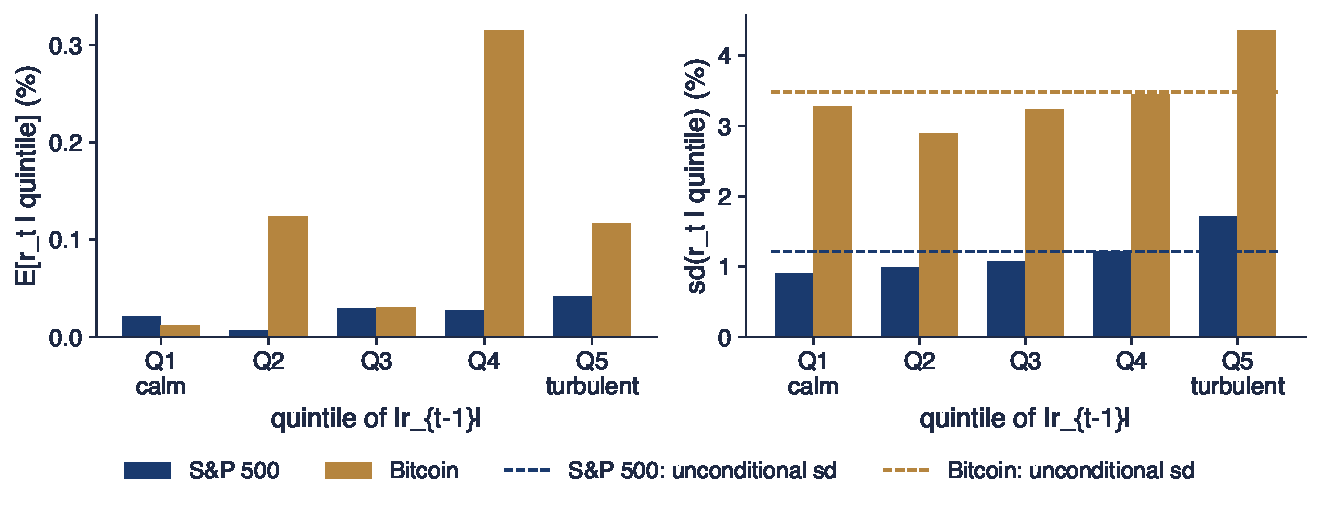
\includegraphics[width=0.97\textwidth,height=0.50\textheight,keepaspectratio]{sfm_ch4_conditional.pdf}
\end{center}
\vspace{-0.25cm}
\begin{itemize}
    \item Quintiles of $|r_{t-1}|$: Q1 = the calmest 20\% of yesterdays, Q5 = the most turbulent 20\%
    \item Conditional mean: between $0.006\%$ and $0.042\%$ for the S\&P 500, no usable pattern
    \item Conditional s.d.: S\&P 500 from 0.91\% (Q1) to 1.71\% (Q5), ratio 1.88; Bitcoin ratio 1.33
    \item Law of total variance, S\&P 500: 1.469 = 1.469 + 0.00013; the between part is 0.01\%
\end{itemize}
\sfmquantlet{Ch_04}{SFM_ch4_dependence}
\end{frame}

\begin{frame}{From Conditional Variance to GARCH}
\itemsize{\footnotesize}
\begin{itemize}
    \item Write the return as $r_t = \mu_t + \sigma_t z_t$, with $z_t$ i.i.d., mean 0, variance 1
    \begin{itemize}
        \item $\mu_t = E[r_t \mid \mathcal{F}_{t-1}]$: the conditional mean, close to constant
        \item $\sigma_t^2 = \text{Var}(r_t \mid \mathcal{F}_{t-1})$: the conditional variance, which changes with the news
    \end{itemize}
    \item ARCH (autoregressive conditional heteroskedasticity) \refEngle: $\sigma_t^2 = \omega + \alpha r_{t-1}^2$
    \begin{itemize}
        \item today's variance is a base level plus a share of yesterday's squared return
        \item $\omega > 0$: the base level; $\alpha \ge 0$: how strongly a large move yesterday raises today's variance
    \end{itemize}
    \item GARCH \refBollerslev: $\sigma_t^2 = \omega + \alpha r_{t-1}^2 + \beta\sigma_{t-1}^2$ (\sfmchlink{https://danpele.github.io/SFM/EN/Courses/chapter9_arch_garch_models.pdf}{Chapter 9})
    \begin{itemize}
        \item $\beta \ge 0$: the persistence; a large $\beta$ keeps a high variance high for many days
    \end{itemize}
    \item Exactly the pattern in the chart: a large $|r_{t-1}|$ raises today's conditional s.d.
    \item The unconditional distribution is a mixture over $\sigma_t$
    \begin{itemize}
        \item it has heavier tails than the Normal distribution, even if $z_t$ is Normal
    \end{itemize}
\end{itemize}
\end{frame}

\begin{frame}{Recap: Conditioning}
\itemsize{\small}
\begin{itemize}
    \item $E[Y \mid X]$ is the best forecast; the tower property averages it back to $E[Y]$
    \item Returns: conditional mean almost flat, conditional variance strongly time-varying
    \item Modelling $\sigma_t^2$ is the job of ARCH and GARCH
\end{itemize}
\end{frame}


%=============================================================================
\section{The Law of Large Numbers and the CLT}
%=============================================================================

\begin{frame}{Two Limit Theorems}
\itemsize{\small}
\begin{itemize}
    \item \textbf{LLN} (law of large numbers): for i.i.d. $X_i$ with $E|X| < \infty$, $\bar X_n \to \mu$ as $n \to \infty$
    \begin{itemize}
        \item $\bar X_n = \frac1n\sum_{i=1}^n X_i$: the sample mean; $\mu = E[X]$: the true mean
        \item the reason why averages, frequencies and Monte Carlo estimates work
    \end{itemize}
    \item \textbf{CLT} (central limit theorem): with finite variance, $\sqrt{n}(\bar X_n - \mu)/\sigma \to N(0, 1)$ (\sfmchlink{https://danpele.github.io/SFM/EN/Courses/chapter2_classical_distributions_stylised_facts.pdf}{Chapter 2})
    \begin{itemize}
        \item the standardised sample mean has, for large $n$, approximately the standard Normal distribution
        \item gives the speed: the error of $\bar X_n$ is about $\sigma/\sqrt{n}$
        \item infinite variance: sums converge to $\alpha$-stable laws instead (\sfmchlink{https://danpele.github.io/SFM/EN/Courses/chapter3_alpha_stable_distributions.pdf}{Chapter 3})
    \end{itemize}
    \item Both need some form of independence; dependent returns converge more slowly
\end{itemize}
\end{frame}

\begin{frame}{The LLN for the Mean Return: Slow}
\itemsize{\footnotesize}
\begin{center}
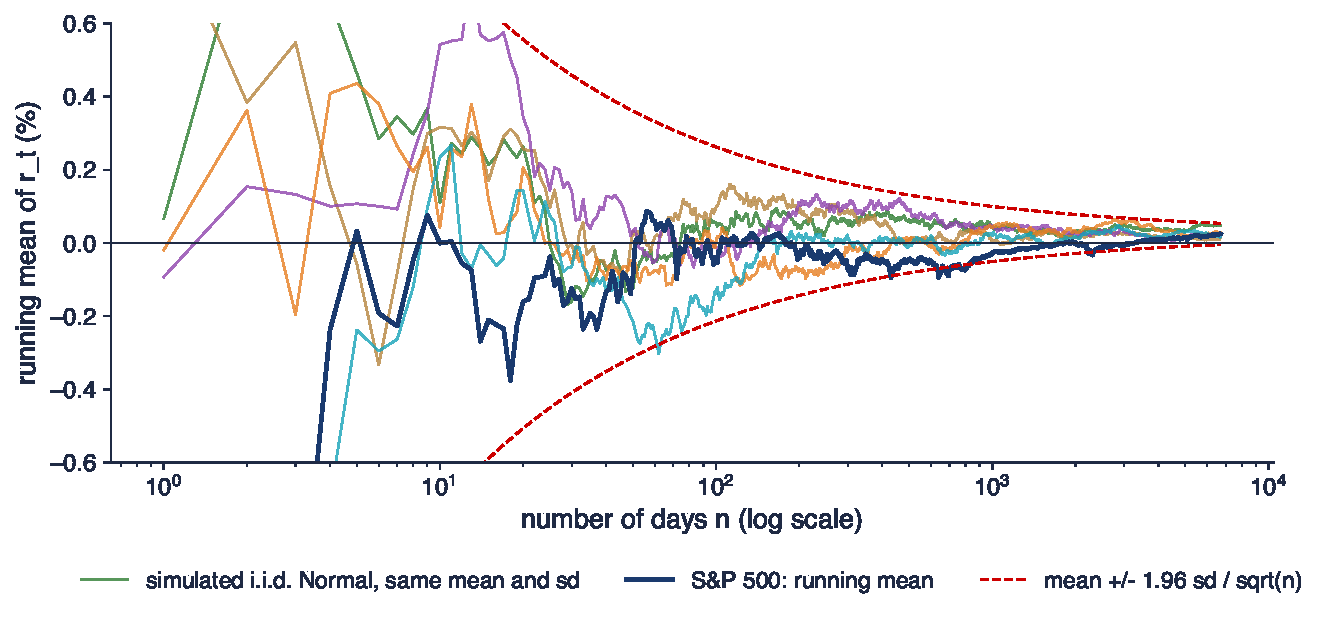
\includegraphics[width=0.97\textwidth,height=0.50\textheight,keepaspectratio]{sfm_ch4_lln.pdf}
\end{center}
\vspace{-0.25cm}
\begin{itemize}
    \item S\&P 500, 26.7 years: mean $0.0247\%$ a day, standard error $\sigma/\sqrt{n} = 0.0148\%$
    \begin{itemize}
        \item $t$ = mean / standard error $= 1.67$; $|t| > 1.96$ would mean a mean significantly different from 0 at 5\%
    \end{itemize}
    \item Annual mean 6.2\%, 95\% interval $[-1.1\%, 13.5\%]$
    \begin{itemize}
        \item even 26 years do not pin down the expected return
        \item for $t = 3$ at this mean and volatility we would need about 86 years of data
    \end{itemize}
\end{itemize}
\sfmquantlet{Ch_04}{SFM_ch4_monte_carlo}
\end{frame}


%=============================================================================
\section{Random Numbers and Monte Carlo}
%=============================================================================

\begin{frame}{The Monte Carlo Idea}
\itemsize{\footnotesize}
\begin{itemize}
    \item Estimate $\theta = E[g(X)]$ by $\hat\theta_N = \frac1N\sum_{i=1}^N g(X_i)$ with simulated $X_i$
    \begin{itemize}
        \item $\theta$: the unknown quantity; $g$: a function of the simulated variable; $N$: the number of simulations
        \item a probability is an expectation: $P(A) = E[\mathbf{1}_A]$, with $\mathbf{1}_A = 1$ if $A$ occurs and 0 otherwise
        \item the LLN makes $\hat\theta_N \to \theta$; the CLT gives the error $\text{sd}(g(X))/\sqrt{N}$
    \end{itemize}
    \item Named after the Monaco casino by Ulam and von Neumann, Los Alamos, 1940s \refMU
    \item In finance \refGlasserman
    \begin{itemize}
        \item prices of path-dependent options, VaR and ES of portfolios, stress scenarios
        \item any expectation without a closed form
    \end{itemize}
    \item Two ingredients: uniform random numbers and a way to turn them into any distribution
\end{itemize}
\end{frame}

\begin{frame}{Pseudo-Random Numbers: Linear Congruential Generators}
\itemsize{\small}
\begin{itemize}
    \item \textbf{LCG} (linear congruential generator): $x_{k+1} = (a x_k + c) \bmod M$, $u_k = x_k/M \in [0, 1)$
    \begin{itemize}
        \item each integer $x_{k+1}$ is computed from the previous one $x_k$
        \item $a$: the multiplier; $c$: the increment; $M$: the modulus; $\bmod M$: the remainder of the division by $M$
        \item $u_k$: the uniform number in $[0, 1)$ obtained by dividing by $M$
    \end{itemize}
    \item Deterministic: the same seed $x_0$ gives the same sequence
    \begin{itemize}
        \item this makes results reproducible
        \item the \textbf{period}: the number of values before the sequence repeats; at most $M$
    \end{itemize}
    \item Real generators use huge $M$; the period must be far longer than any simulation
\end{itemize}
\end{frame}

\begin{frame}{Worked Example: an LCG with $M = 16$}
\itemsize{\small}
\begin{itemize}
    \item SFErangen1: $a = 5$, $c = 1$, $M = 16$, $x_0 = 7$
    \begin{itemize}
        \item first step: $x_1 = (5 \times 7 + 1) \bmod 16 = 36 \bmod 16 = 4$
        \item the sequence $x$: 7, 4, 5, 10, 3, 0, 1, 6, 15, 12, 13, 2, 11, 8, 9, 14, 7
    \end{itemize}
    \item Period 16, the maximum possible, $M$
    \begin{itemize}
        \item with $a = 4$ the sequence sticks after one step (period 1)
    \end{itemize}
    \item Good uniform marginals are not enough
    \begin{itemize}
        \item consecutive numbers must also look independent: the next chart
    \end{itemize}
\end{itemize}
\end{frame}

\begin{frame}{RANDU: Random Numbers Fall Mainly in the Planes (SFErandu)}
\itemsize{\footnotesize}
\begin{center}
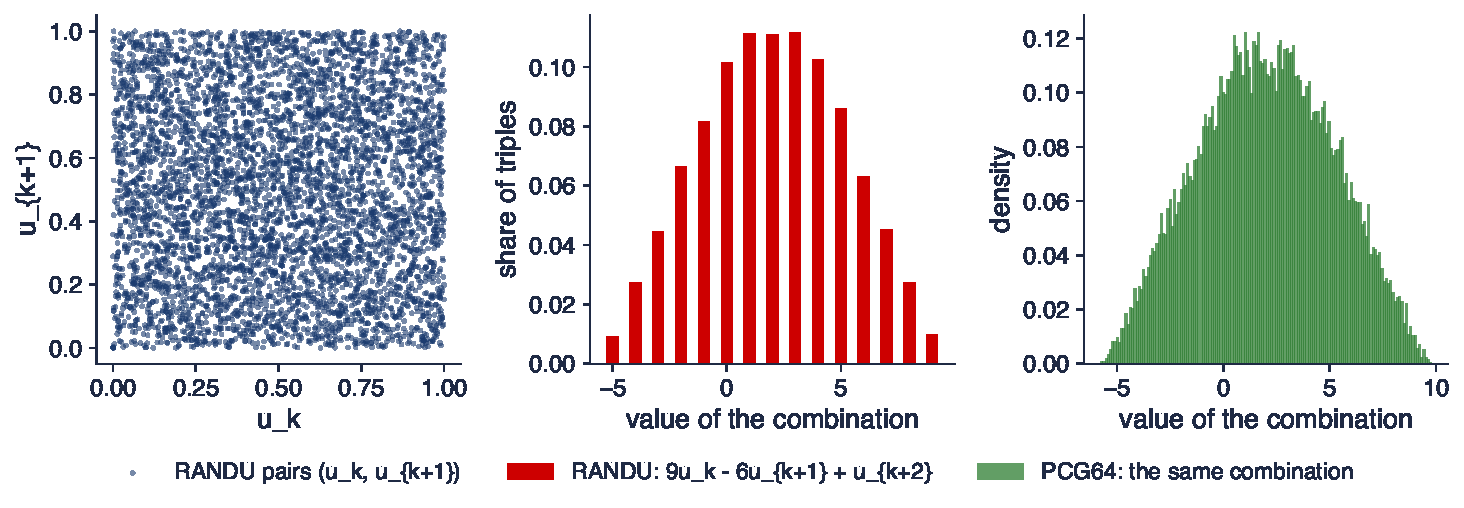
\includegraphics[width=0.97\textwidth,height=0.52\textheight,keepaspectratio]{sfm_ch4_randu.pdf}
\end{center}
\vspace{-0.25cm}
\begin{itemize}
    \item RANDU, IBM, 1960s: $x_{k+1} = 65539\,x_k \bmod 2^{31}$; pairs look uniform (left), correlation $0.003$
    \item But $9u_k - 6u_{k+1} + u_{k+2}$ takes only 15 integer values, from -5 to 9: all triples lie on 15 planes \refMarsaglia
    \item Modern generators: Mersenne Twister \refMT, PCG64 (the NumPy default, right panel)
\end{itemize}
\sfmquantlet{Ch_04}{SFM_ch4_random_numbers}
\end{frame}

\begin{frame}{The Inverse Transform Method}
\itemsize{\footnotesize}
\begin{itemize}
    \item \textbf{Theorem}: if $U \sim U(0, 1)$ and $F$ is a CDF, then $X = F^{-1}(U)$ has CDF $F$
    \begin{itemize}
        \item $U(0, 1)$: the uniform distribution on $[0, 1]$, so $P(U \le u) = u$
        \item in words: a uniform number, read as a probability, is turned into the quantile of that order
        \item proof: $P(X \le x) = P(F^{-1}(U) \le x) = P(U \le F(x)) = F(x)$
    \end{itemize}
    \item Exponential with rate $\lambda > 0$: $F(x) = 1 - e^{-\lambda x}$, so $X = -\ln(1 - U)/\lambda$
    \begin{itemize}
        \item obtained by solving $u = F(x)$ for $x$; the mean is $1/\lambda$
        \item $\lambda = 2$, $u = 0.9$: $x = -\ln(0.1)/2 = 1.151$
    \end{itemize}
    \item Normal: $X = \mu + \sigma\,\Phi^{-1}(U)$
    \begin{itemize}
        \item $\Phi^{-1}$: the quantile function of $N(0, 1)$; $\mu$, $\sigma$: the desired mean and standard deviation
    \end{itemize}
    \item Data: use the empirical quantile function $\hat F^{-1}$
    \begin{itemize}
        \item this is resampling past days: historical simulation and the bootstrap
    \end{itemize}
\end{itemize}
\end{frame}

\begin{frame}{Inverse Transform: Exponential, Normal and Historical}
\itemsize{\footnotesize}
\begin{center}
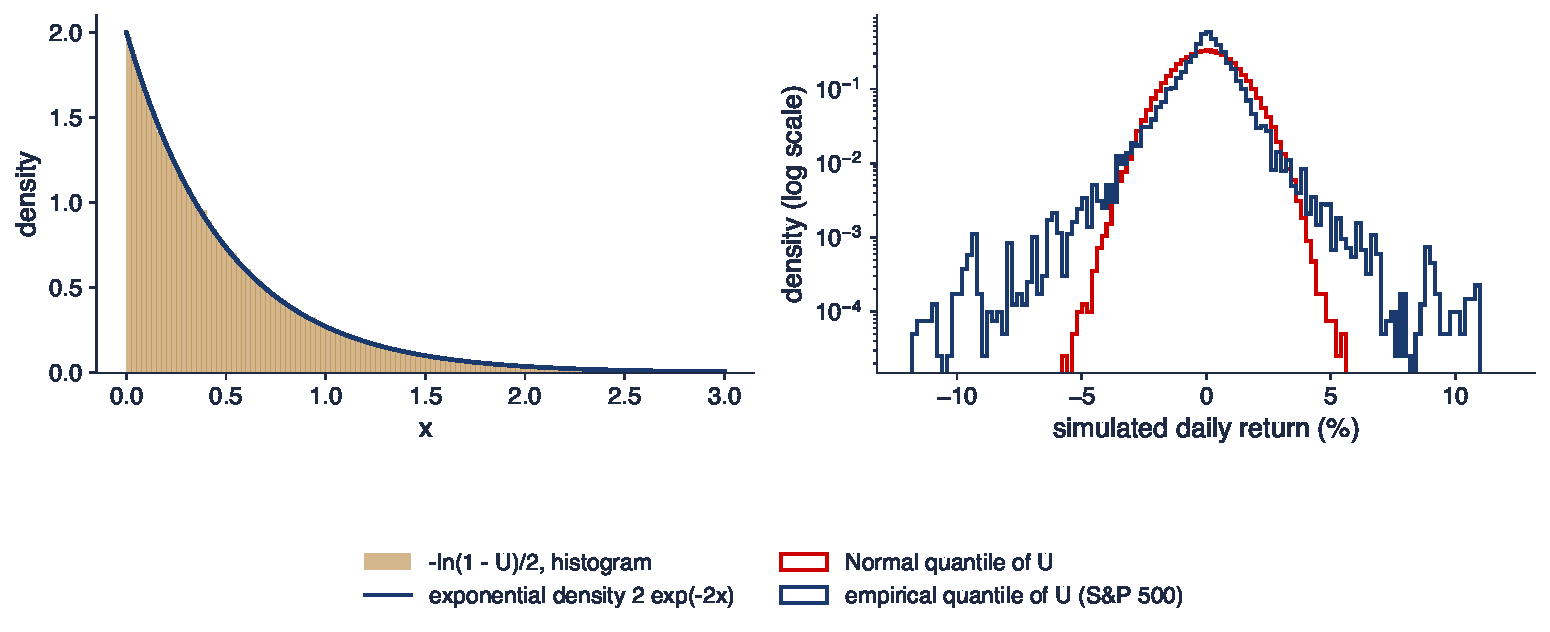
\includegraphics[width=0.97\textwidth,height=0.52\textheight,keepaspectratio]{sfm_ch4_inverse_transform.pdf}
\end{center}
\vspace{-0.25cm}
\begin{itemize}
    \item Left: 200\,000 draws $-\ln(1 - U)/2$ match the exponential density; sample mean 0.500 (theory $1/\lambda = 0.5$)
    \item Right: the same uniforms through the Normal and the empirical S\&P 500 quantile functions
    \item Draws below $-5\%$: 0.0035\% Normal vs 0.34\% historical (data: 0.34\%); worst draw -5.7\% vs -12.7\%
\end{itemize}
\sfmquantlet{Ch_04}{SFM_ch4_random_numbers}
\end{frame}

\begin{frame}{Worked Example: a Monthly Loss Probability by Monte Carlo (1/2)}
\itemsize{\small}
\begin{itemize}
    \item Model: S\&P 500 daily log returns i.i.d. $N(0.0247, 1.213^2)$, in \%
    \begin{itemize}
        \item $N(m, s^2)$: the Normal distribution with mean $m$ and variance $s^2$
    \end{itemize}
    \item Event: the 21-day log return (one month) is below $-10\%$
    \begin{itemize}
        \item $p$: its probability, the quantity we want
    \end{itemize}
    \item Exact: the sum of 21 i.i.d. Normal returns is $N(0.519, 5.56^2)$
    \begin{itemize}
        \item mean $21 \times 0.0247$, standard deviation $1.213\sqrt{21}$
        \item standardise: $z = (-10 - 0.519)/5.56 = -1.892$
        \item $p = \Phi(z) = 2.922\%$, with $\Phi$ the CDF of $N(0, 1)$
    \end{itemize}
\end{itemize}
\end{frame}

\begin{frame}{Worked Example: a Monthly Loss Probability by Monte Carlo (2/2)}
\itemsize{\small}
\begin{itemize}
    \item Monte Carlo: simulate $N$ months; $\hat p_N$ = share of simulated months below $-10\%$
    \begin{itemize}
        \item standard error $\sqrt{p(1 - p)/N}$: the typical distance between $\hat p_N$ and $p$
    \end{itemize}
    \item Results
    \begin{itemize}
        \item $N = 1\,000$: $3.000\%$ (s.e. 0.533\%)
        \item $N = 100\,000$: $2.901\%$ (s.e. 0.053\%)
        \item 10 times more precision needs 100 times more simulations
    \end{itemize}
    \item For a relative error of 10\% at the 95\% level: $N \approx 1.96^2(1 - p)/(0.1^2 p) = 12\,762$
    \begin{itemize}
        \item obtained from $1.96 \times \sqrt{p(1 - p)/N} = 0.1\,p$: the half-width of the interval is 10\% of $p$
        \item a rare event needs many simulations
    \end{itemize}
\end{itemize}
\end{frame}

\begin{frame}{Monte Carlo Converges at Rate $1/\sqrt{N}$}
\itemsize{\footnotesize}
\begin{center}
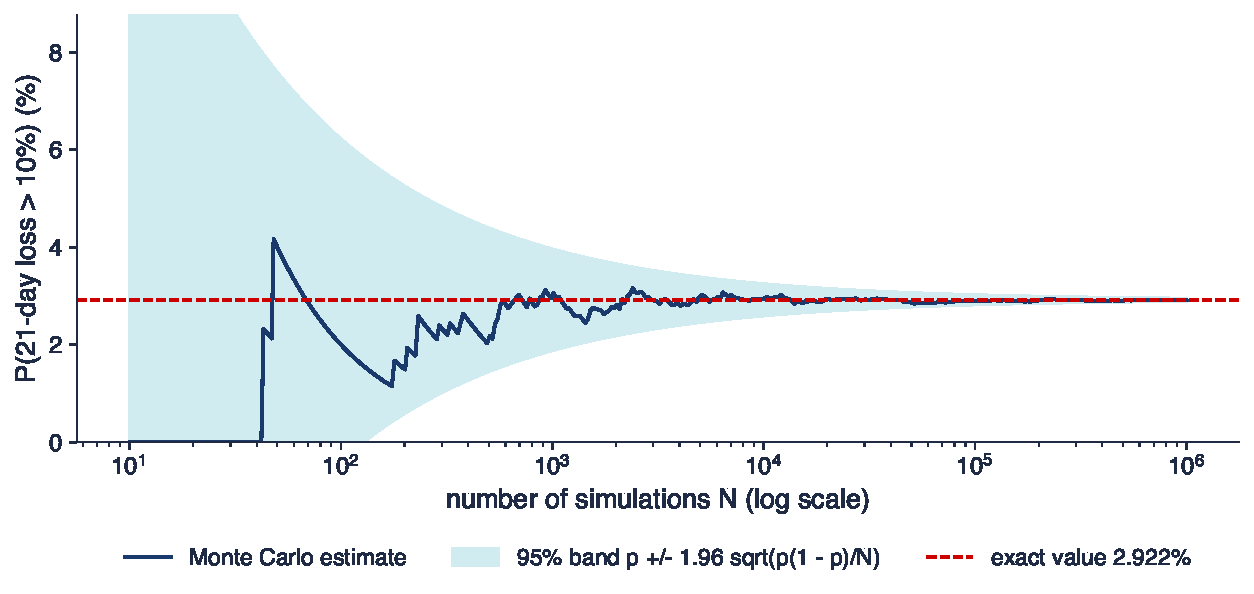
\includegraphics[width=0.97\textwidth,height=0.56\textheight,keepaspectratio]{sfm_ch4_monte_carlo.pdf}
\end{center}
\vspace{-0.25cm}
\begin{itemize}
    \item The estimate wanders for small $N$ and settles inside the 95\% band, which shrinks like $1/\sqrt{N}$
    \item $N = 10^6$: $2.926\%$ vs exact 2.922\%, s.e. 0.017\%
    \item Monte Carlo removes the simulation error, not the model error: Seminar 4 (B3) repeats it with resampled days
\end{itemize}
\sfmquantlet{Ch_04}{SFM_ch4_monte_carlo}
\end{frame}

\begin{frame}{Recap: Random Numbers and Monte Carlo}
\itemsize{\small}
\begin{itemize}
    \item Pseudo-random generators are deterministic; check them in several dimensions
    \item $F^{-1}(U)$ turns uniforms into any distribution, including the empirical one
    \item Monte Carlo error $\propto 1/\sqrt{N}$; always report it
\end{itemize}
\end{frame}


%=============================================================================
\section{The Binomial Model}
%=============================================================================

\begin{frame}{The Binomial Process}
\itemsize{\footnotesize}
\begin{itemize}
    \item Each period the price is multiplied by $u$ (up) with probability $p$, or by $d < u$ (down) with probability $1 - p$
    \begin{itemize}
        \item $u$, $d$: the up and down factors (e.g. $u = 1.2$: $+20\%$); the periods are independent
    \end{itemize}
    \item After $n$ steps with $K$ up moves: $S_n = S_0 u^K d^{n - K}$
    \begin{itemize}
        \item $S_0$: the initial price; $K \sim B(n, p)$: the number of up moves is binomial
        \item $\ln S_n = \ln S_0 + K\ln u + (n - K)\ln d$: a random walk in log prices (Section 9)
    \end{itemize}
    \item $E[S_n] = S_0\,(pu + (1 - p)d)^n$, because the steps are independent
    \begin{itemize}
        \item $pu + (1 - p)d$: the expected growth factor of one step
        \item the basis of the binomial option pricing model \refCRR; textbook: \refFHH, Ch.~7
    \end{itemize}
\end{itemize}
\end{frame}

\begin{frame}{Worked Example: a Two-Step Tree}
\itemsize{\footnotesize}
\begin{itemize}
    \item $S_0 = 100$, $u = 1.2$, $d = 0.8$, $p = 0.6$
    \item Terminal values and probabilities
    \begin{itemize}
        \item $uu$: 144 with $p^2 = 0.36$; $ud$ or $du$: 96 with $2p(1-p) = 0.48$; $dd$: 64 with $(1-p)^2 = 0.16$
    \end{itemize}
    \item $E[S_2] = 100 \times (0.6 \times 1.2 + 0.4 \times 0.8)^2 = 100 \times 1.04^2 = 108.16$
    \item $P(S_2 < 100) = 0.48 + 0.16$
    \begin{itemize}
        \item one up and one down move lose money, because $ud = 0.96 < 1$
    \end{itemize}
    \item With $p^* = (1 - d)/(u - d) = 0.50$ the price is a fair game: $E[S_{t+1} \mid S_t] = S_t$ (Section 9)
    \begin{itemize}
        \item $p^*$ solves $p^*u + (1 - p^*)d = 1$: the expected growth factor of a step equals 1
    \end{itemize}
\end{itemize}
\end{frame}

\begin{frame}{Calibrating the Tree to a Market (Cox--Ross--Rubinstein)}
\itemsize{\footnotesize}
\begin{itemize}
    \item \textbf{CRR} (Cox--Ross--Rubinstein) with step $\Delta t$: $u = e^{\sigma\sqrt{\Delta t}}$, $d = 1/u$, $p = (e^{\mu\Delta t} - d)/(u - d)$
    \begin{itemize}
        \item $\Delta t$: the length of one step, in years; $\mu$: the annual drift; $\sigma$: the annual volatility
        \item $d = 1/u$: an up move followed by a down move returns to the start
        \item chosen so that the mean and the variance of each step match a market with drift $\mu$ and volatility $\sigma$
    \end{itemize}
    \item S\&P 500, 2000--2026: $\sigma = 19.23\%$, $\mu = 8.06\%$ a year; daily steps, $\Delta t = 1/252$
    \begin{itemize}
        \item $u = 1.0122$, $d = 0.9880$, $p = 0.5102$
    \end{itemize}
    \item As $\Delta t \to 0$, $\ln S_T$ becomes Normal (CLT for $K$)
    \begin{itemize}
        \item $T$: the horizon; the tree converges to GBM (Section 10)
    \end{itemize}
\end{itemize}
\end{frame}

\begin{frame}{Binomial Paths and the Lognormal Limit (SFEBinomp)}
\itemsize{\footnotesize}
\begin{center}
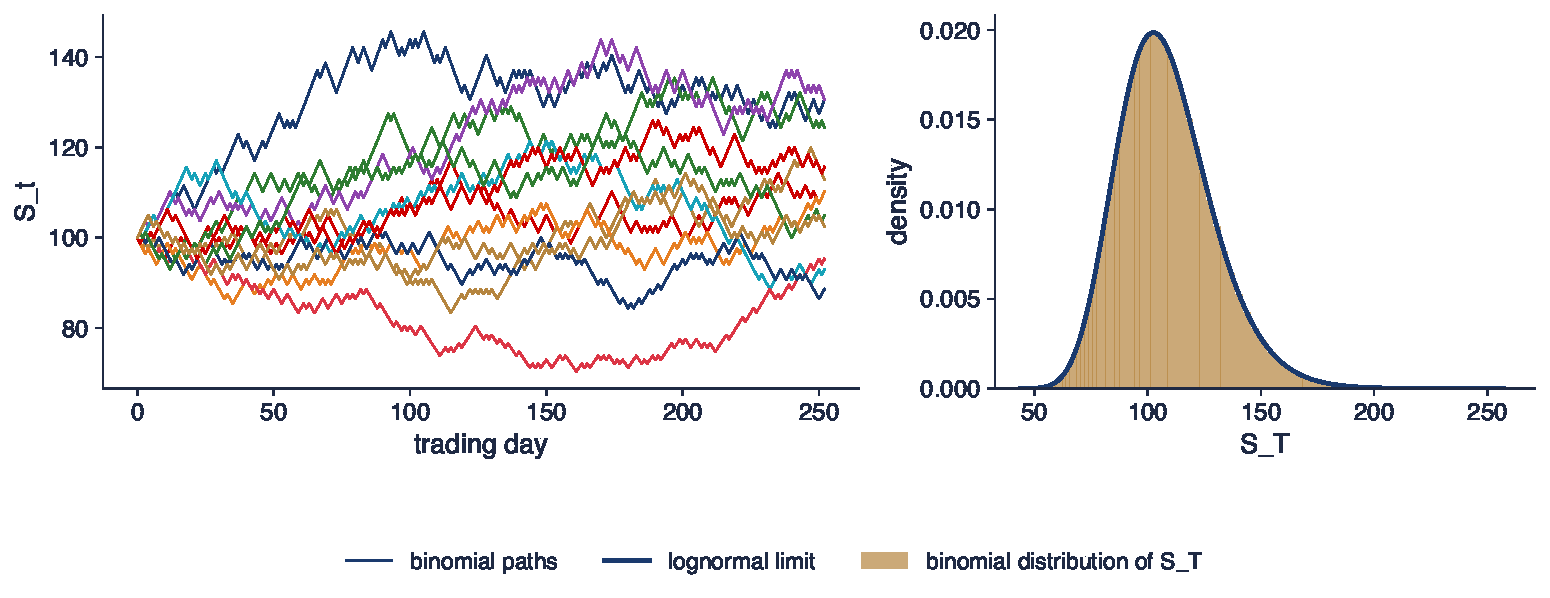
\includegraphics[width=0.97\textwidth,height=0.46\textheight,keepaspectratio]{sfm_ch4_binomial.pdf}
\end{center}
\vspace{-0.25cm}
\begin{itemize}
    \item Left: 12 paths over one year of daily steps, $S_0 = 100$
    \item Right: distribution of $S_T$ after 252 steps ($T = 1$ year); $E[S_T] = 108.40$ $= 100e^{\mu}$
    \begin{itemize}
        \item 5\% quantile 78.5 vs 77.6 in the lognormal limit
    \end{itemize}
    \item $P(S_T < 100)$: 39.7\% binomial vs 37.3\% lognormal
    \begin{itemize}
        \item the exact value $S_T = 100$ has a positive probability, which the binomial counts on one side only
    \end{itemize}
\end{itemize}
\sfmquantlet{Ch_04}{SFM_ch4_binomial}
\end{frame}

\begin{frame}{Recap: The Binomial Model}
\itemsize{\small}
\begin{itemize}
    \item Up or down each period: $S_n = S_0 u^K d^{n-K}$ with binomial $K$
    \item CRR matches $\mu$ and $\sigma$; the limit is lognormal
    \item A special $p^*$ turns the price into a fair game: the key to option pricing
\end{itemize}
\end{frame}


%=============================================================================
\section{Discrete-Time Stochastic Processes}
%=============================================================================

\begin{frame}{Stochastic Processes and Information}
\itemsize{\small}
\begin{itemize}
    \item A \textbf{stochastic process} $\{X_t\}$: a family of random variables indexed by time
    \begin{itemize}
        \item one realisation = one path; a price series is a single path of the process
    \end{itemize}
    \item $\mathcal{F}_t$: the information available at time $t$ (past prices, news)
    \begin{itemize}
        \item it grows with $t$: nothing is forgotten (a \textbf{filtration})
    \end{itemize}
    \item \textbf{(Weakly) stationary}: $E[X_t]$ and $\text{Cov}(X_t, X_{t+h})$ do not depend on $t$
    \begin{itemize}
        \item $h$: the lag between two dates; the mean and the dependence look the same at every date
        \item returns: roughly yes; prices: no
    \end{itemize}
    \item Textbook: \refFHH, Ch.~4 and Sec.~11.3
\end{itemize}
\end{frame}

\begin{frame}{White Noise and the Random Walk}
\itemsize{\footnotesize}
\begin{itemize}
    \item \textbf{White noise}: $E[\varepsilon_t] = 0$, $\text{Var}(\varepsilon_t) = \sigma^2$, $\text{Cov}(\varepsilon_t, \varepsilon_s) = 0$ for $t \ne s$
    \begin{itemize}
        \item $\varepsilon_t$: the shock at time $t$; mean zero, constant variance $\sigma^2$, no correlation across dates
        \item i.i.d. noise is stronger: the $\varepsilon_t$ are independent, not only uncorrelated
    \end{itemize}
    \item \textbf{Random walk}: $S_t = S_{t-1} + \mu + \varepsilon_t = S_0 + \mu t + \sum_{s=1}^t \varepsilon_s$
    \begin{itemize}
        \item each step adds the drift $\mu$ and a new shock; $S_0$: the starting value
        \item $E[S_t] = S_0 + \mu t$; $\text{Var}(S_t) = t\sigma^2$ grows with $t$: not stationary
        \item simulated with $\sigma = 1$: variance 10.1, 49.8, 100.9 at $t = 10, 50, 100$
    \end{itemize}
    \item Log prices as a random walk = returns as white noise
    \begin{itemize}
        \item the benchmark of \sfmchlink{https://danpele.github.io/SFM/EN/Courses/chapter7_efficient_markets_random_walk_vr.pdf}{Chapter 7} (efficient markets)
    \end{itemize}
\end{itemize}
\end{frame}

\begin{frame}{Martingales}
\itemsize{\footnotesize}
\begin{itemize}
    \item $\{X_t\}$ is a \textbf{martingale} if $E|X_t| < \infty$ and $E[X_{t+1} \mid \mathcal{F}_t] = X_t$
    \begin{itemize}
        \item $E|X_t| < \infty$: the mean exists; $\mathcal{F}_t$: the information up to $t$
        \item a fair game: the best forecast of tomorrow is today
    \end{itemize}
    \item A \textbf{martingale difference}: $\varepsilon_t = X_t - X_{t-1}$ with $E[\varepsilon_t \mid \mathcal{F}_{t-1}] = 0$
    \begin{itemize}
        \item the change cannot be predicted from the past
    \end{itemize}
    \item Examples
    \begin{itemize}
        \item a random walk without drift; $S_t^2 - t\sigma^2$ for the same walk; the binomial price under $p^*$
    \end{itemize}
    \item Martingale $\ne$ i.i.d. increments: the conditional \textbf{variance} may change, as in GARCH
    \begin{itemize}
        \item the efficient-market idea in its weak form \refFama: excess returns are a martingale difference
    \end{itemize}
\end{itemize}
\end{frame}

\begin{frame}{The AR(1) Process}
\itemsize{\footnotesize}
\begin{itemize}
    \item \textbf{AR(1)} (autoregressive of order 1): $X_t = c + \phi X_{t-1} + \varepsilon_t$, $\varepsilon_t$ white noise
    \begin{itemize}
        \item today's value is a constant, plus a share $\phi$ of yesterday's value, plus a new shock
        \item $c$: the constant; $\phi$: the persistence; $\sigma^2$: the variance of $\varepsilon_t$
        \item $\phi = 0$: white noise; $\phi = 1$, $c = \mu$: random walk
    \end{itemize}
    \item Stationary iff $|\phi| < 1$; then
    \begin{itemize}
        \item mean $c/(1 - \phi)$, variance $\sigma^2/(1 - \phi^2)$
        \item autocorrelation at lag $h$: $\rho(h) = \text{Corr}(X_t, X_{t-h}) = \phi^h$, decaying geometrically
        \item half-life of a shock: $\ln 0.5/\ln\phi$ periods, the time until half of a shock is gone
    \end{itemize}
    \item Uses
    \begin{itemize}
        \item interest rates and spreads (mean reversion)
        \item the squared returns behave like a persistent AR, which leads to GARCH
    \end{itemize}
\end{itemize}
\end{frame}

\begin{frame}{The AR(1) Process: Simulation}
\itemsize{\small}
\begin{itemize}
    \item Simulated with $\sigma = 1$, $\phi = 0.5$
    \begin{itemize}
        \item variance 1.34 (theory $1/(1 - 0.5^2) = 1.33$)
        \item $\rho(5) = 0.034$ (theory $0.5^5 = 0.031$); half-life 1.0 periods
    \end{itemize}
    \item Simulated with $\sigma = 1$, $\phi = 0.95$
    \begin{itemize}
        \item variance 10.20 (theory 10.26)
        \item $\rho(5) = 0.772$; half-life 13.5 periods
    \end{itemize}
    \item The closer $\phi$ is to 1, the larger the variance and the slower a shock fades
\end{itemize}
\end{frame}

\begin{frame}{White Noise, AR(1) and Random Walk, Same Shocks}
\itemsize{\footnotesize}
\begin{center}
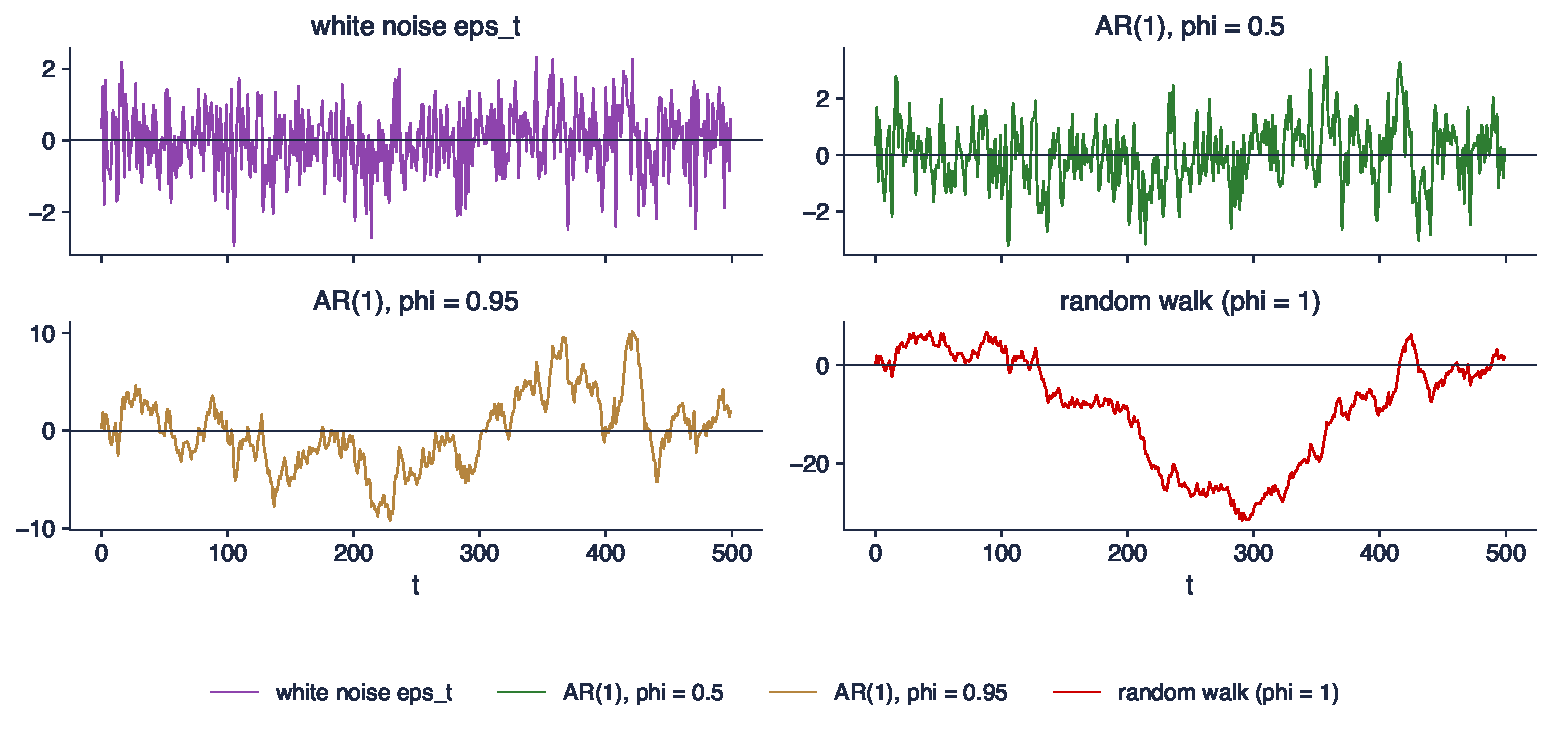
\includegraphics[width=0.97\textwidth,height=0.58\textheight,keepaspectratio]{sfm_ch4_processes.pdf}
\end{center}
\vspace{-0.25cm}
\begin{itemize}
    \item The larger $\phi$, the longer a shock lives: the AR(1) with $\phi = 0.95$ wanders, but returns to 0
    \item The random walk never returns on purpose: shocks are permanent and its variance grows with $t$
\end{itemize}
\sfmquantlet{Ch_04}{SFM_ch4_processes}
\end{frame}

\begin{frame}{Question for the Room: Which One Is Real?}
\itemsize{\footnotesize}
\begin{center}
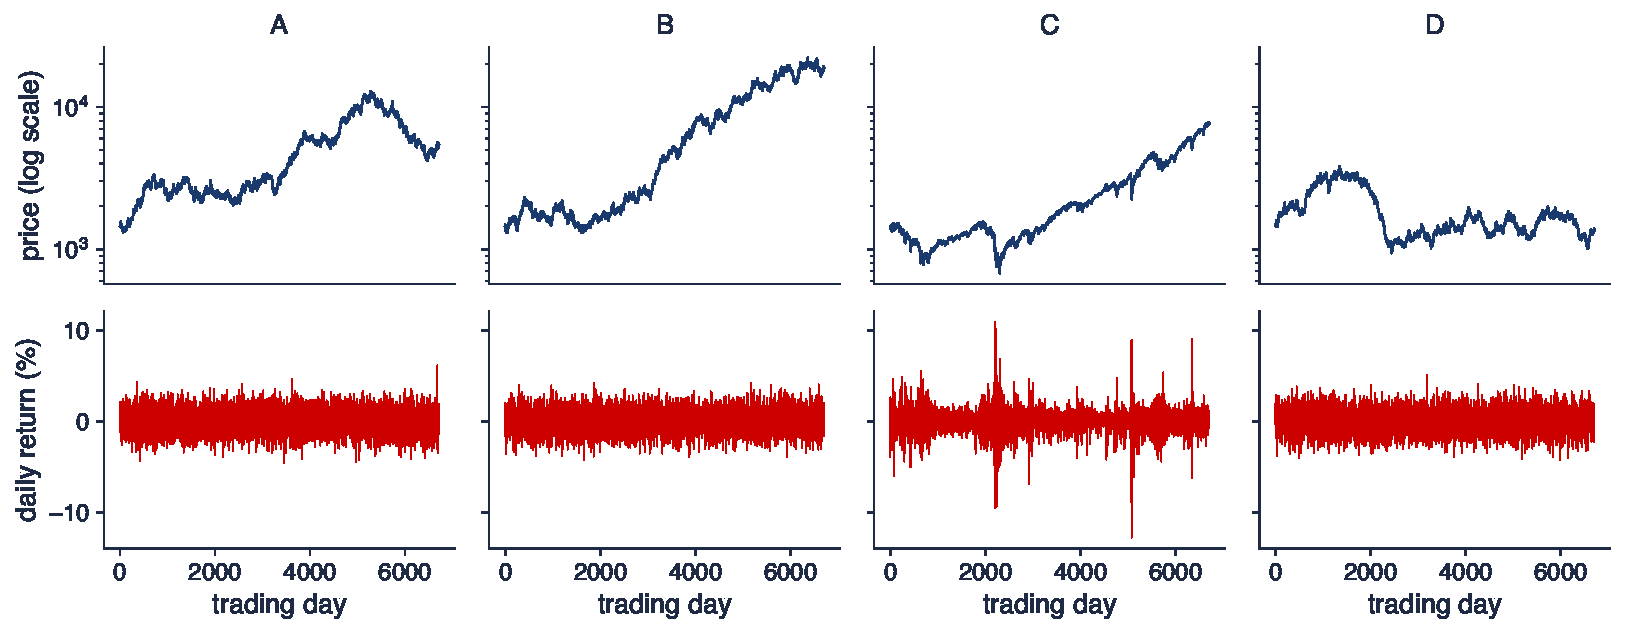
\includegraphics[width=0.97\textwidth,height=0.56\textheight,keepaspectratio]{sfm_ch4_spot_the_real.pdf}
\end{center}
\vspace{-0.25cm}
\begin{itemize}
    \item One column is the S\&P 500, 2000--2026; three are GBM paths (i.i.d. Normal returns) with the same mean and volatility
    \item \textbf{What do you think?} Which column is real, from the prices alone?
    \item \textbf{What do you think?} Which column is real, from the returns?
\end{itemize}
\sfmquantlet{Ch_04}{SFM_ch4_processes}
\end{frame}

\begin{frame}{Answer: Column C}
\itemsize{\small}
\begin{itemize}
    \item \textbf{Answer}: column C is the S\&P 500
    \item Prices: hard to tell; random walks with drift produce booms and long falls too
    \begin{itemize}
        \item this is why \refBachelier{} and \refOsborne{} modelled prices as random walks
    \end{itemize}
    \item Returns: obvious; the real series has quiet years and violent clusters (2008, 2020)
    \begin{itemize}
        \item excess kurtosis 10.7 vs at most 0.02 in the simulations; $\text{Corr}(r_t^2, r_{t-1}^2) = 0.31$ vs at most 0.006
        \item largest absolute daily move 12.8\% vs 6.2\%
    \end{itemize}
    \item Lesson: a model can fit the price path and still be wrong about risk
\end{itemize}
\end{frame}

\begin{frame}{Recap: Discrete-Time Processes}
\itemsize{\small}
\begin{itemize}
    \item White noise: uncorrelated; i.i.d. noise: independent; a martingale difference: unpredictable mean
    \item Random walk: permanent shocks, variance $t\sigma^2$; AR(1) with $|\phi| < 1$: shocks fade at rate $\phi^h$
    \item Prices look like random walks; returns are not i.i.d.
\end{itemize}
\end{frame}


%=============================================================================
\section{The Wiener Process and Geometric Brownian Motion}
%=============================================================================

\begin{frame}{From Pollen to Prices: Brownian Motion}
\itemsize{\footnotesize}
\begin{columns}[T]
\begin{column}{0.60\textwidth}
\begin{itemize}
    \item 1827: the botanist Robert Brown sees pollen particles jiggling in water
    \item 1900: Louis Bachelier models the Paris bond market with the same motion, five years before physics \refBachelier
    \item 1905: Albert Einstein explains it by molecular collisions \refEinstein
    \item 1923: Norbert Wiener builds the rigorous mathematical object \refWiener
    \item 1959: \refOsborne{} applies it to log prices: geometric Brownian motion
\end{itemize}
\end{column}
\begin{column}{0.36\textwidth}
\begin{center}
\centering
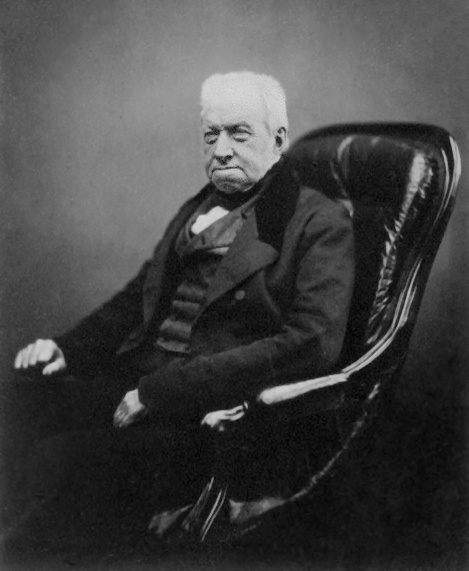
\includegraphics[height=0.20\textheight]{ch4_brown_1855.jpg}\\[1mm]
\imgcap{Robert Brown (1773--1858)}
\imgcredit{https://commons.wikimedia.org/wiki/File:Robert_Brown_(botanist).jpg}{Photo: Maull \& Polyblank (1855); public domain; Wikimedia Commons}\\[2mm]
\centering
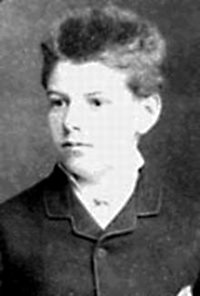
\includegraphics[height=0.20\textheight]{ch0_bachelier.jpg}\\[1mm]
\imgcap{Louis Bachelier (1870--1946)}
\imgcredit{https://commons.wikimedia.org/wiki/File:LouisBachelier.jpg}{Photo: unknown author; public domain; Wikimedia Commons}
\end{center}
\end{column}
\end{columns}
\end{frame}

\begin{frame}{The Wiener Process}
\itemsize{\footnotesize}
\begin{columns}[T]
\begin{column}{0.64\textwidth}
\begin{itemize}
    \item $\{W(t), t \ge 0\}$ is a \textbf{Wiener process} (standard Brownian motion) if
    \begin{itemize}
        \item $W(0) = 0$
        \item increments over disjoint intervals are independent
        \item $W(t) - W(s) \sim N(0, t - s)$ for $s < t$: the variance equals the elapsed time
        \item the paths are continuous
    \end{itemize}
    \item Limit of the scaled random walk $W_n(t) = (\varepsilon_1 + \dots + \varepsilon_{\lfloor nt\rfloor})/\sqrt{n}$ (Donsker)
    \begin{itemize}
        \item $\varepsilon_i = \pm 1$ with probability $1/2$ each; $n$ steps per unit of time
        \item $\lfloor nt\rfloor$: the number of steps up to time $t$ (integer part); dividing by $\sqrt{n}$ keeps the variance equal to $t$
    \end{itemize}
    \item Textbook: \refFHH, Ch.~5
\end{itemize}
\end{column}
\begin{column}{0.32\textwidth}
\centering
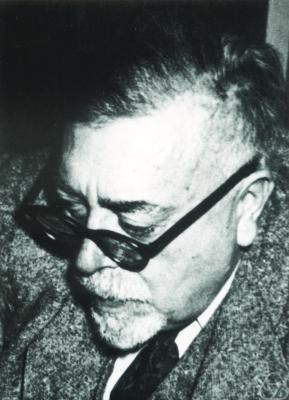
\includegraphics[height=0.50\textheight]{ch4_wiener.jpg}\\[1mm]
\imgcap{Norbert Wiener (1894--1964)}
\imgcredit{https://commons.wikimedia.org/wiki/File:Norbert_wiener.jpg}{Photo: Konrad Jacobs; CC BY-SA 2.0 DE; Wikimedia Commons}
\end{column}
\end{columns}
\end{frame}

\begin{frame}{From Random Walks to the Wiener Process (SFEWienerProcess)}
\itemsize{\footnotesize}
\begin{center}
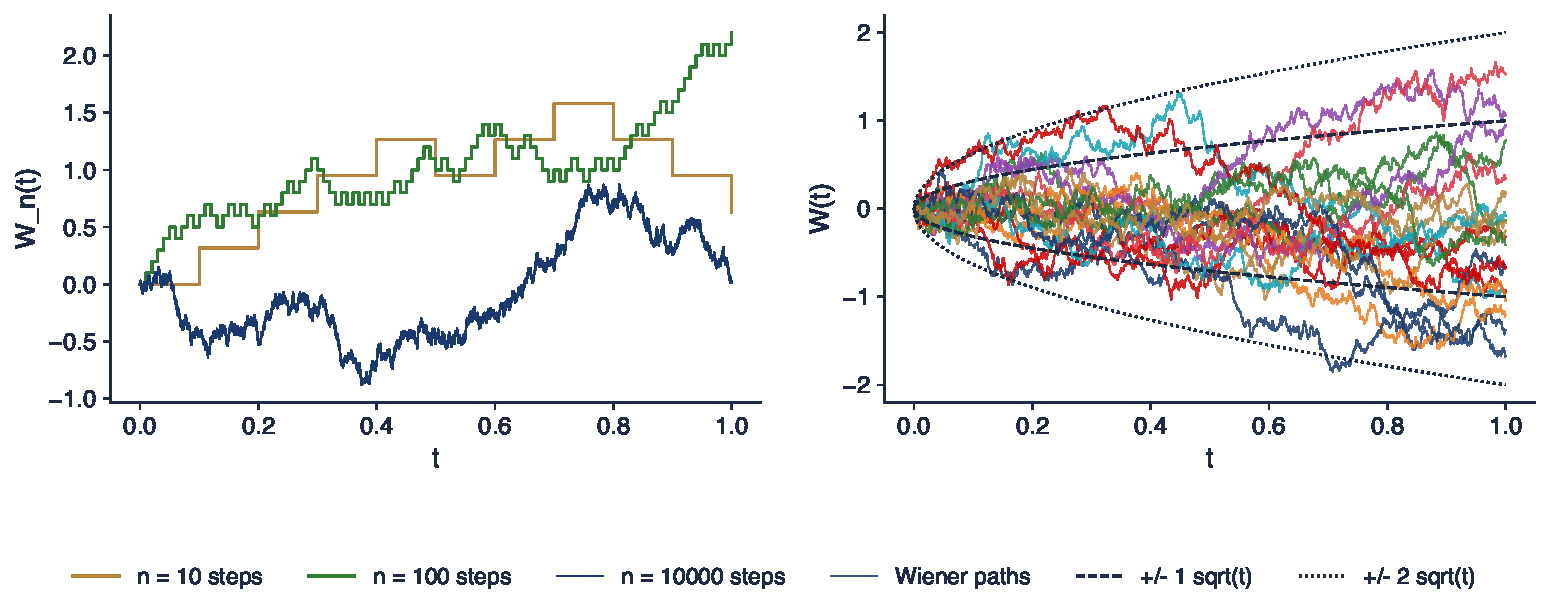
\includegraphics[width=0.97\textwidth,height=0.50\textheight,keepaspectratio]{sfm_ch4_wiener.pdf}
\end{center}
\vspace{-0.25cm}
\begin{itemize}
    \item Left: scaled random walks with 10, 100 and 10\,000 steps; the steps vanish, the randomness stays
    \item Right: 20 Wiener paths; $\text{Var}(W(t)) = t$, so they spread like $\pm\sqrt{t}$
    \begin{itemize}
        \item simulated $\text{Var}(W(1)) = 1.006$; 68.2\% of $W(1)$ inside $\pm 1$ (theory 68.3\%)
    \end{itemize}
\end{itemize}
\sfmquantlet{Ch_04}{SFM_ch4_wiener_gbm}
\end{frame}

\begin{frame}{Strange Properties of Wiener Paths}
\itemsize{\footnotesize}
\begin{itemize}
    \item Continuous everywhere, differentiable nowhere
    \begin{itemize}
        \item the slope $(W(t + h) - W(t))/h \sim N(0, 1/h)$ has a variance $1/h$ that grows without bound as $h \to 0$
    \end{itemize}
    \item \textbf{Quadratic variation}: $\sum_k (W(t_{k+1}) - W(t_k))^2 \to t$ on a finer and finer grid
    \begin{itemize}
        \item $0 = t_0 < t_1 < \dots < t$: the grid; the sum of squared increments tends to the elapsed time $t$
        \item 1000 steps on $[0, 1]$: mean 0.999, s.d. 0.045 across 10\,000 paths
        \item the reason why $(dW)^2 = dt$ in It\^o calculus, and why realised variance measures volatility (\sfmchlink{https://danpele.github.io/SFM/EN/Courses/chapter8_volatility_estimators.pdf}{Chapter 8})
    \end{itemize}
    \item $\text{Cov}(W(s), W(t)) = \min(s, t)$: simulated $\text{Cov}(W(0.5), W(1)) = 0.496$
    \item $W$ is a martingale; so is $W(t)^2 - t$
\end{itemize}
\end{frame}

\begin{frame}{Geometric Brownian Motion}
\itemsize{\footnotesize}
\begin{itemize}
    \item \textbf{GBM} (geometric Brownian motion): $dS_t = \mu S_t\,dt + \sigma S_t\,dW_t$
    \begin{itemize}
        \item $dS_t$: the change of the price over a very short interval $dt$
        \item $dW_t$: the increment of the Wiener process over $dt$, distributed $N(0, dt)$
        \item the relative change $dS/S$ has drift $\mu$ and volatility $\sigma$, both per year
    \end{itemize}
    \item Solution: $S_t = S_0\exp\big((\mu - \sigma^2/2)t + \sigma W_t\big)$
    \begin{itemize}
        \item $\ln(S_t/S_0) \sim N\big((\mu - \sigma^2/2)t, \sigma^2 t\big)$
        \item lognormal prices, i.i.d. Normal log returns
    \end{itemize}
    \item The model behind \refBS{} (\sfmchlink{https://danpele.github.io/SFM/EN/Courses/chapter6_model_selection_risk_management.pdf}{Chapter 6} of the textbook)
\end{itemize}
\end{frame}

\begin{frame}{GBM: Mean, Median and Simulation}
\itemsize{\small}
\begin{itemize}
    \item Mean $E[S_t] = S_0e^{\mu t}$; median $S_0e^{(\mu - \sigma^2/2)t}$
    \begin{itemize}
        \item the median is lower: half of the paths end below $S_0e^{(\mu - \sigma^2/2)t}$
        \item the gap, $\sigma^2/2$ a year in log terms, is the volatility drag
    \end{itemize}
    \item Exact simulation on a grid: $S_{t + \Delta t} = S_t\exp\big((\mu - \sigma^2/2)\Delta t + \sigma\sqrt{\Delta t}\,Z\big)$
    \begin{itemize}
        \item $\Delta t$: the grid step, in years; $Z \sim N(0, 1)$, a new independent draw at each step
        \item exact because each log increment is Normal with the right mean and variance
    \end{itemize}
\end{itemize}
\end{frame}

\begin{frame}{GBM Calibrated to the S\&P 500 (SFEsimGBM)}
\itemsize{\footnotesize}
\begin{center}
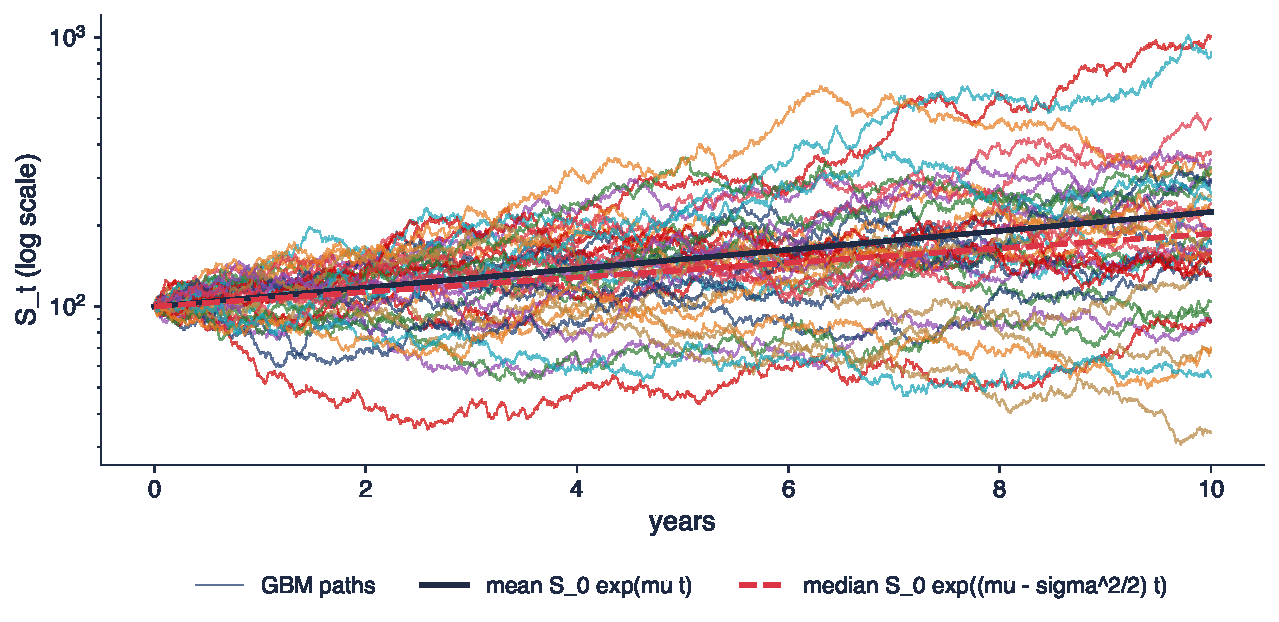
\includegraphics[width=0.97\textwidth,height=0.54\textheight,keepaspectratio]{sfm_ch4_gbm_paths.pdf}
\end{center}
\vspace{-0.25cm}
\begin{itemize}
    \item Calibration, 2000--2026: $\sigma = 19.23\%$, log drift $\mu - \sigma^2/2 = 6.21\%$, so $\mu = 8.06\%$ a year
    \item After $T = 10$ years: mean 224.0, median 186.2
    \begin{itemize}
        \item 62.0\% of the paths end below the mean; theory: $\Phi(\sigma\sqrt{T}/2) = 61.9\%$, with $\Phi$ the $N(0, 1)$ CDF
    \end{itemize}
    \item Probability of a loss after 10 years: 15.3\%
\end{itemize}
\sfmquantlet{Ch_04}{SFM_ch4_wiener_gbm}
\end{frame}

\begin{frame}{Real Paths in the GBM Fan}
\itemsize{\scriptsize}
\begin{center}
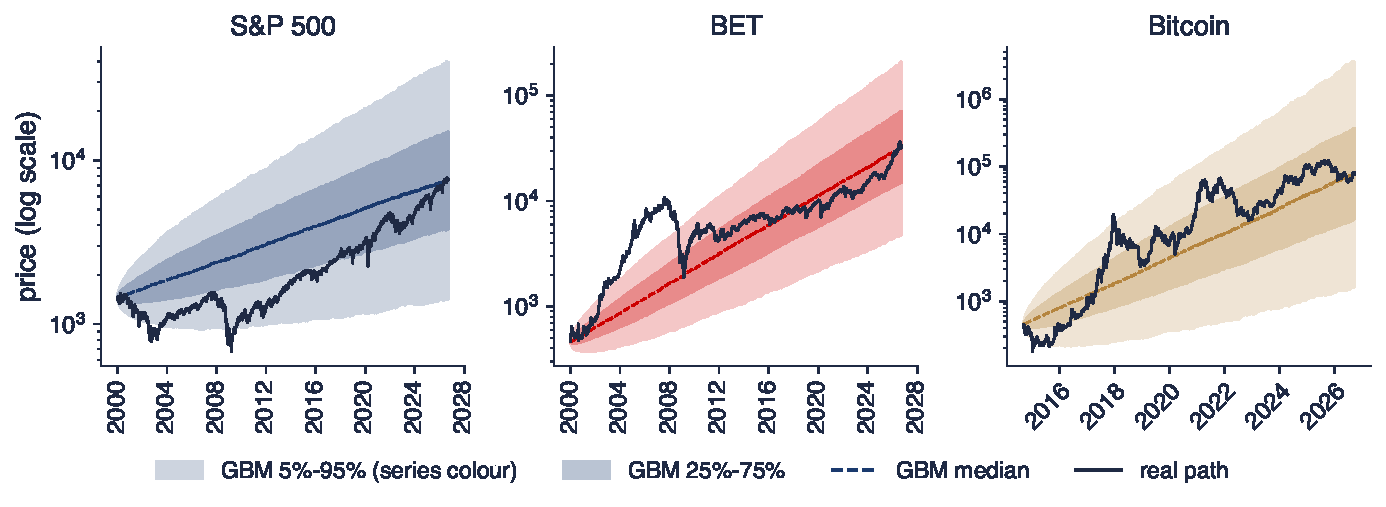
\includegraphics[width=0.97\textwidth,height=0.46\textheight,keepaspectratio]{sfm_ch4_gbm_fan.pdf}
\end{center}
\vspace{-0.25cm}
\begin{itemize}
    \item Each fan: 4000 GBM paths with the drift and volatility of the series itself, started on its first day
    \item S\&P 500: the path reached the 0.5\% quantile on 23 July 2002, then the median at the end
    \begin{itemize}
        \item outside the 90\% band 7\% of the time
    \end{itemize}
    \item BET: outside the band 24\% of the time
    \begin{itemize}
        \item the 2000--2007 boom and the 2008 crash are not GBM-like
        \item Bitcoin: $\sigma = 66.6\%$ a year makes the fan enormous
    \end{itemize}
\end{itemize}
\sfmquantlet{Ch_04}{SFM_ch4_wiener_gbm}
\end{frame}

\begin{frame}{What GBM Misses}
\itemsize{\scriptsize}
\begin{center}
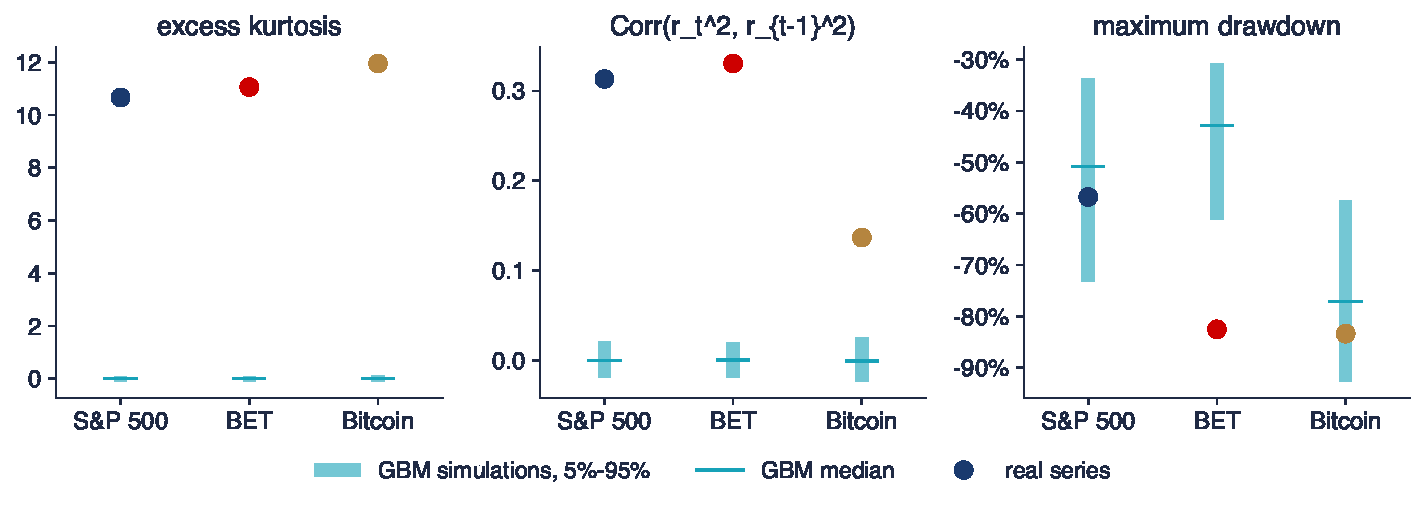
\includegraphics[width=0.97\textwidth,height=0.46\textheight,keepaspectratio]{sfm_ch4_gbm_check.pdf}
\end{center}
\vspace{-0.25cm}
\begin{itemize}
    \item Excess kurtosis: S\&P 500 10.7, BET 11.1, Bitcoin 12.0; 90\% of 300 GBM simulations lie within $[-0.10, 0.09]$
    \item Volatility clustering: $\text{Corr}(r_t^2, r_{t-1}^2) = 0.31$, $0.33$, $0.14$ vs at most $0.03$ under GBM
    \item Maximum drawdown: S\&P 500 -57\% is ordinary for GBM; BET -83\% is beyond all but 5\% of the paths (5\% quantile -61\%)
    \item 4-sigma days: 46 (S\&P 500) vs at most 1 in 95\% of the GBM paths; crypto has the same problem \refPeleCrypto
\end{itemize}
\sfmquantlet{Ch_04}{SFM_ch4_wiener_gbm}
\end{frame}

\begin{frame}{Recap: Wiener Process and GBM}
\itemsize{\small}
\begin{itemize}
    \item Wiener process: independent Normal increments with variance equal to the elapsed time
    \item GBM: lognormal prices, median below mean, the benchmark of option pricing
    \item Real returns have heavy tails and volatility clusters that GBM cannot produce
\end{itemize}
\end{frame}


%=============================================================================
\section{AI for Scientific Discovery}
%=============================================================================

\begin{frame}{An Open Question: Does GBM Get Drawdown Risk Right?}
\itemsize{\scriptsize}
\begin{center}
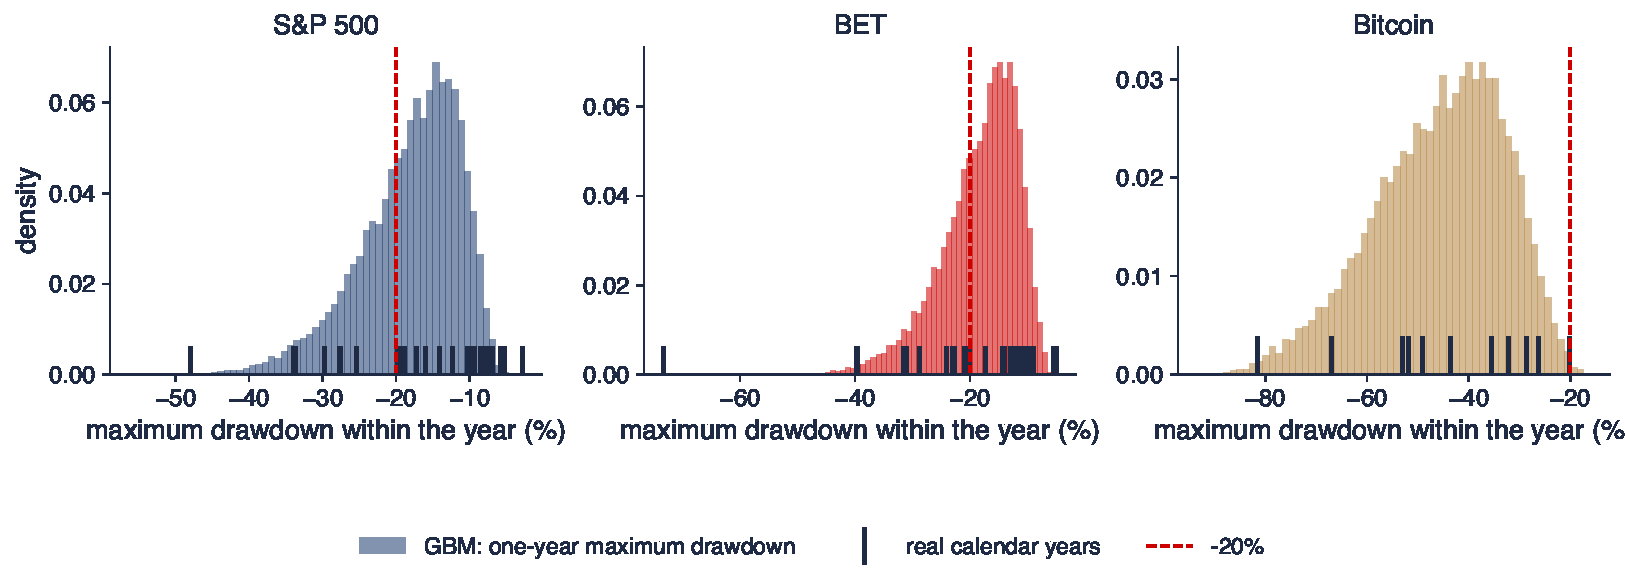
\includegraphics[width=0.97\textwidth,height=0.42\textheight,keepaspectratio]{sfm_ch4_drawdown_years.pdf}
\end{center}
\vspace{-0.25cm}
\begin{itemize}
    \item Drawdown: the fall from the highest price reached so far; here, within a calendar year
    \begin{itemize}
        \item beyond 20\%: S\&P 500 in 6 of 26 years (23\%) vs 34\% under GBM; BET 46\% vs 34\%
    \end{itemize}
    \item Beyond 40\%: GBM expects 0.14 such years for the S\&P 500 and 0.17 for the BET
    \begin{itemize}
        \item both had 1 (2008: -48\% and -73\%)
    \end{itemize}
    \item Open question
    \begin{itemize}
        \item does GBM overstate moderate drawdowns and understate extreme ones because calm and crisis years cluster?
    \end{itemize}
\end{itemize}
\sfmquantlet{Ch_04}{SFM_ch4_drawdown_open}
\end{frame}

\begin{frame}{How AI Could Help}
\itemsize{\footnotesize}
\begin{itemize}
    \item \textbf{Literature}: find studies of drawdown distributions and of their link to volatility clustering, and summarise them
    \item \textbf{Code}: draft simulations of yearly drawdowns under GBM, the i.i.d. bootstrap and a GARCH model
    \item \textbf{Design}: propose a test that compares the observed number of bad years with the model probability
    \item Example prompt
    \begin{itemize}
        \item \aiprompt{Write Python code that simulates 10,000 one-year paths of daily S\&P 500 returns under GBM and under an i.i.d. bootstrap of 2000-2026 returns, and returns the probability of a drawdown beyond 20\% and 40\% within the year.}
    \end{itemize}
\end{itemize}
\end{frame}

\begin{frame}{What to Check}
\itemsize{\small}
\begin{itemize}
    \item Definitions: drawdown from the running peak within the year, not from the first day of the year
    \item Calibration: the same $\mu$ and $\sigma$, the same number of trading days a year as the data
    \item Inference: 26 years is a small sample; compute a binomial p-value, not only shares
    \item Mechanism: the i.i.d. bootstrap keeps heavy tails but removes clustering; the difference isolates the effect of clustering
    \item References: every cited paper must exist; check the DOI
\end{itemize}
\end{frame}

\begin{frame}{Project Seed}
\itemsize{\small}
\begin{itemize}
    \item \textbf{Question}: how wrong is GBM about the probability of a bad year, and why?
    \begin{itemize}
        \item data: S\&P 500, DAX, BET and Bitcoin from the course data
    \end{itemize}
    \item Steps
    \begin{itemize}
        \item compute within-year maximum drawdowns for every calendar year
        \item simulate the same statistic under GBM, the i.i.d. bootstrap and a GARCH(1,1) model (\sfmchlink{https://danpele.github.io/SFM/EN/Courses/chapter9_arch_garch_models.pdf}{Chapter 9})
        \item compare the shares beyond 20\% and 40\% with binomial tests
    \end{itemize}
    \item Deliverable: one table, one chart, and a paragraph on what the data can and cannot show
    \item Declare any AI use, and list the errors of the AI that you corrected \refWang
\end{itemize}
\end{frame}


%=============================================================================
\section{Summary}
%=============================================================================

\begin{frame}{Key Takeaways}
\itemsize{\small}
\begin{itemize}
    \item Distributions: PMF, PDF, CDF and quantiles; VaR 1\% is minus a quantile
    \item Covariance drives portfolio risk; uncorrelated returns are not independent
    \item Conditional variance changes with yesterday's news: the starting point of GARCH
    \item Monte Carlo: inverse transform plus the LLN; error $\propto 1/\sqrt{N}$
    \item Binomial tree $\to$ GBM; random walk, martingale, white noise, AR(1)
    \item GBM fits price paths roughly, but misses heavy tails, clustering and extreme drawdowns
\end{itemize}
\end{frame}

\begin{frame}{Key Formulas}
\itemsize{\small}
\begin{center}
\footnotesize
\begin{tabular}{ll}
\toprule
\textbf{Quantity} & \textbf{Formula} \\
\midrule
Variance of a sum & $\text{Var}(aX + bY) = a^2\sigma_X^2 + b^2\sigma_Y^2 + 2ab\,\text{Cov}(X, Y)$ \\
Correlation & $\rho = \text{Cov}(X, Y)/(\sigma_X\sigma_Y)$ \\
Tower property & $E[E[Y \mid X]] = E[Y]$ \\
Total variance & $\text{Var}(Y) = E[\text{Var}(Y \mid X)] + \text{Var}(E[Y \mid X])$ \\
Inverse transform & $X = F^{-1}(U)$, $U \sim U(0, 1)$ \\
Monte Carlo error & $\sqrt{p(1 - p)/N}$ \\
Random walk & $S_t = S_{t-1} + \mu + \varepsilon_t$, $\text{Var}(S_t) = t\sigma^2$ \\
AR(1) & $\text{Var}(X_t) = \sigma^2/(1 - \phi^2)$, $\rho(h) = \phi^h$ \\
GBM & $S_t = S_0\exp((\mu - \sigma^2/2)t + \sigma W_t)$, $E[S_t] = S_0e^{\mu t}$ \\
\bottomrule
\end{tabular}
\end{center}
\end{frame}

\begin{frame}{Check Yourself}
\itemsize{\small}
\begin{itemize}
    \item \textbf{Question}: $\sigma_1 = 2\%$, $\sigma_2 = 3\%$, $\rho = 0.5$; what is the volatility of the 50/50 portfolio?
    \begin{itemize}
        \item \textbf{Answer}: $\sqrt{0.25 \times 4 + 0.25 \times 9 + 2 \times 0.25 \times 0.5 \times 2 \times 3} = \sqrt{4.75} = 2.18\%$
    \end{itemize}
    \item \textbf{Question}: GBM with $\mu = 8\%$, $\sigma = 20\%$, $S_0 = 100$; what are the mean and the median of $S_1$?
    \begin{itemize}
        \item \textbf{Answer}: mean $100e^{0.08} = 108.33$, median $100e^{0.06} = 106.18$
    \end{itemize}
    \item \textbf{Question}: AR(1) with $\phi = 0.8$ and $\sigma = 1$; what is its variance?
    \begin{itemize}
        \item \textbf{Answer}: $1/(1 - 0.64) = 2.78$
    \end{itemize}
    \item Next: \sfmchlink{https://danpele.github.io/SFM/EN/Courses/chapter5_heavy_tails_evt.pdf}{Chapter 5}, heavy tails and extreme value theory
\end{itemize}
\end{frame}


%=============================================================================
\section{References}
%=============================================================================

\begin{frame}{References (1/2)}
\itemsize{\tiny}
\begin{itemize}
    \item Bachelier, L. (1900). \href{https://doi.org/10.24033/asens.476}{Théorie de la spéculation}. \textit{Annales scientifiques de l'École Normale Supérieure}, 17, 21--86.
    \item Black, F., Scholes, M. (1973). \href{https://doi.org/10.1086/260062}{The pricing of options and corporate liabilities}. \textit{Journal of Political Economy}, 81(3), 637--654.
    \item Bollerslev, T. (1986). \href{https://doi.org/10.1016/0304-4076(86)90063-1}{Generalized autoregressive conditional heteroskedasticity}. \textit{Journal of Econometrics}, 31(3), 307--327.
    \item Borak, S., Härdle, W.K., López-Cabrera, B. (2013). \href{https://doi.org/10.1007/978-3-642-33929-5}{\textit{Statistics of Financial Markets: Exercises and Solutions}}, 2nd ed. Springer.
    \item Cont, R. (2001). \href{https://doi.org/10.1080/713665670}{Empirical properties of asset returns: stylized facts and statistical issues}. \textit{Quantitative Finance}, 1(2), 223--236.
    \item Cox, J.C., Ross, S.A., Rubinstein, M. (1979). \href{https://doi.org/10.1016/0304-405X(79)90015-1}{Option pricing: a simplified approach}. \textit{Journal of Financial Economics}, 7(3), 229--263.
    \item Einstein, A. (1905). \href{https://doi.org/10.1002/andp.19053220806}{Über die von der molekularkinetischen Theorie der Wärme geforderte Bewegung von in ruhenden Flüssigkeiten suspendierten Teilchen}. \textit{Annalen der Physik}, 322(8), 549--560.
    \item Engle, R.F. (1982). \href{https://doi.org/10.2307/1912773}{Autoregressive conditional heteroscedasticity with estimates of the variance of United Kingdom inflation}. \textit{Econometrica}, 50(4), 987--1007.
    \item Fama, E.F. (1970). \href{https://doi.org/10.2307/2325486}{Efficient capital markets: a review of theory and empirical work}. \textit{Journal of Finance}, 25(2), 383--417.
    \item Franke, J., Härdle, W.K., Hafner, C.M. (2019). \href{https://doi.org/10.1007/978-3-030-13751-9}{\textit{Statistics of Financial Markets: An Introduction}}, 5th ed. Springer.
\end{itemize}
\end{frame}

\begin{frame}{References (2/2)}
\itemsize{\tiny}
\begin{itemize}
    \item Glasserman, P. (2003). \href{https://doi.org/10.1007/978-0-387-21617-1}{\textit{Monte Carlo Methods in Financial Engineering}}. Springer.
    \item Kolmogoroff, A. (1933). \href{https://doi.org/10.1007/978-3-642-49888-6}{\textit{Grundbegriffe der Wahrscheinlichkeitsrechnung}}. Springer, Berlin.
    \item Marsaglia, G. (1968). \href{https://doi.org/10.1073/pnas.61.1.25}{Random numbers fall mainly in the planes}. \textit{Proceedings of the National Academy of Sciences}, 61(1), 25--28.
    \item Matsumoto, M., Nishimura, T. (1998). \href{https://doi.org/10.1145/272991.272995}{Mersenne twister: a 623-dimensionally equidistributed uniform pseudo-random number generator}. \textit{ACM Transactions on Modeling and Computer Simulation}, 8(1), 3--30.
    \item Metropolis, N., Ulam, S. (1949). \href{https://doi.org/10.1080/01621459.1949.10483310}{The Monte Carlo method}. \textit{Journal of the American Statistical Association}, 44(247), 335--341.
    \item Osborne, M.F.M. (1959). \href{https://doi.org/10.1287/opre.7.2.145}{Brownian motion in the stock market}. \textit{Operations Research}, 7(2), 145--173.
    \item Pele, D.T., Wesselhöfft, N., Härdle, W.K., Kolossiatis, M., Yatracos, Y.G. (2023). \href{https://doi.org/10.1080/1351847X.2021.1960403}{Are cryptos becoming alternative assets?} \textit{European Journal of Finance}, 29(10), 1064--1105.
    \item Wang, H., Fu, T., Du, Y., Gao, W., et al. (2023). \href{https://doi.org/10.1038/s41586-023-06221-2}{Scientific discovery in the age of artificial intelligence}. \textit{Nature}, 620, 47--60.
    \item Wiener, N. (1923). \href{https://doi.org/10.1002/sapm192321131}{Differential-space}. \textit{Journal of Mathematics and Physics}, 2(1--4), 131--174.
\end{itemize}
\end{frame}

\end{document}
